\documentclass[dvipdfmx]{newthesis}

\usepackage{graphicx} % dvipdfmxオプションを指定しないでください
\hyperrefsetpdfmetadata
\addbibresource{reference.bib}
\usepackage{bxjalipsum}
\usepackage{amsmath,amssymb}
\usepackage{mathtools}
\usepackage{enumerate}


\title{離散事象システムに基づいた人間と調和したマルチロボットによる倉庫自動化に関する研究}
% \engtitle{Sample of Resume Template}
\date{令和2年度}
\affiliation{
  大阪市立大学 工学部 電気情報工学科 \\
  エレクトロニクス領域
}
\author{野田 健太朗}


\begin{document}


% 0.表紙
\maketitle

% 0.1.概要
\begin{abstract}
    物流業界の人手不足とさらに2020年に流行した感染症の影響で世界中でネットショッピングの利用率の増加\cite{soumu}に伴って,無人搬送ロボットを導入した倉庫自動化による作業の効率化が進んでいる.
    
    しかし,すべてロボットだけで完結する完全な倉庫の自動化の実現は困難である.無人搬送ロボットは荷物をピッキングして運搬する機能はあっても,予期せぬトラブルが発生した場合,それを対処することが難しい.また,ロボットには,さまざまな大きさや形のもののピッキング,及び想定されていなかったタスクを処理することが困難である.
    
    ここで,近年注目されている,自動化された一環のシステムに人間を介入させたシステムを考えるHuman-in-the-Loopという概念を取り入れることで,手先の器用さ,問題解決能力などの人間の強みと,正確性,パワーやスピードなどのロボットの強みをかけ合わせることにより予期せぬ事態に対応できると考えた.従来では倉庫内のトラブルを解決処理しに人間が立ち入るとき,自動化されたシステムを停止していたが,人間をシステムの一部と考えることでロボットの動作中にトラブルを処理できるようにする.
    
    このとき人間の安全を確保したシステムをつくる必要があり,その制御方法について,人間の経路のロボットの使用を禁止する方法と,人間にロボットを接近させない方法を提案する.
    また,ケーススタデによって検証し,2つの方法が有効であり,人間の安全を確保できることを示した.
    
\end{abstract}

 \pagenumbering{roman}
% 0.2.本文の目次
\tableofcontents
%\thesisstyleindex

% 0.3.図の目次
\listoffigures

% 0.4.表の目次
\listoftables

% 1.序論
\chapter{序論}\label{chap:intro}
 \pagenumbering{arabic}
 \setcounter{page}{1}
 
\section{背景}
%注釈\cite{キーワード}。\\
近年,実店舗に出向かなくても買い物ができるネットショッピングが増加している.

さらに,2020年に入ってからCOVID-19の影響もあり,さらに拍車をかけるようにネットショッピングが買い物の主流な形になるようになった.それにより,物流業界では人手不足が深刻化している.それを解決するのが移動式ロボットによる倉庫の自動化である.それはつまり,人が目的の荷物を探すため歩き回る必要があったが,その仕事をロボットが代わりに行うということである.このように倉庫内で無人で荷物を運搬するロボットを活用することが,労働の削減につながり,さらには労働者不足を解消することにつながる.

倉庫内のロボットを制御するうえで,ロボット同士の衝突,ロボットで道がふさがれていまいお互い身動きができなくなるデッドロック状態などの問題が考えられる.それらの問題を解決する有効な方法として,離散事象システムのスーパーバイザ制御が挙げられる\cite{Supervisory_Control}\cite{Supervisory_Control_2}.

先行研究に,スーパーバイザ制御の計算に特化したTCTという計算ソフトウェアを使用して,自動化倉庫のスーパーバイザ制御を設計する研究がある\cite{Pre_research}.これは,ロボットごとの動的オートマトンモデルを作り,衝突やブロッキング状態が発生してしまうロボットの動きを制限して,タスクを各ロボットが円滑にこなせるように,スーパーバイザを計算するアルゴリズムが提案されている.

倉庫自動化の実用化において,ロボットで対応できないトラブルが発生したとき,どう対処するかが課題となっている.現在,そのようなトラブルが発生して,処理するために人が立ち入るとなると,自動化されたシステムを完全に停止させなければならない.これは効率化を目指すうえで解決しなければならない問題である.

\section{目的}
本研究では,システムを停止せずに,人間が倉庫に立ち入ることを想定したケースにおいても,離散事象システムを用いたスーパーバイザ制御を応用できることを追究する.倉庫内で発生した予測不可能なトラブルを人間が処理するとき,ロボットも使用する通路を通りトラブルの起こった場所まで行かなければならない.つまり,人間も考慮したうえでロボットの制御を行わなくてはならない.このように,自動化された一環のシステムに,人間を介入させてシステムを構築するHuman-in-the-loopという近年注目を浴びており,センシングや機械学習などさまざまな分野で応用されている\cite{HITLref_1}\cite{HITLref_2}\cite{HITLref_3}\cite{HITLref_4}.本研究では倉庫の自動化にこの考えを取り入れた.

人間がロボットの動き回る倉庫内に入る制御を考えるとき,最も重要なのは人間の絶対的な安全を確保しなければならないということである.ロボットが通常通りせかせかと運搬している倉庫内に人間が立ち入るのは危険で,人間の安全な領域を確保しなければならない\cite{JISD6802}.
予期せぬトラブルや特殊な作業など,人間が行わなければならないタスクが発生したとき,自動化されたシステムを完全に停止することなく処理するには,人の安全を保障できるロボットの制御が求められる.
そのため,人の安全を条件とした倉庫内の荷物運搬ロボットの制御をHuman-in-the-loopの考えを取り入れたスーパーバイザ制御理論で考える.

論文の構成は次のようになっている.第2章は,スーパーバイザ制御理論の基礎を述べる.第3章は,倉庫の自動化についてモデリングし,スーパーバイザ制御理論を適応させる方法を紹介する.第4章は,人間を考慮したシステムを制御する方法を2つ提案して説明する.第5章では,シミュレーションを行い,システムの安全性について検証する.第6章は,まとめと今後の課題について述べる.
\clearpage

% 2.
\chapter{スーパーバイザ制御理論}
%またスーパーバイザ制御とは,制御対象に対して,制御要求を満たさない遷移をしてしまう事象を起こらないように禁止するシステムである.
この章では,離散事象システムとオートマトン,およびスーパーバイザ制御の計算方法を解説する.

\section{オートマトン}

\subsection{有限オートマトンの基本}

離散事象システムとは,離散的な状態集合を持つ事象駆動型システムである\cite{DES}.事象が生起すると,その事象に依存して状態が変わり,その状態が時間的に持続するのが特徴である.
オペーションシステム,データベースシステム,通信システム,生産システム,シーケンス制御システムなどが離散事象システムとみなせるいい例である\cite{des_example}.

離散事象システムのモデリングには有限オートマトンが適している.有限オートマトンとは有限個の状態と事象が定義されている動的システムのことである.生起した事象と状態遷移関数に従って,現在いる状態を遷移し連続する一連の動作(ふるまい)をモデリングする.

有限オートマトン$G$は次のように5つの要素から表される.
\begin{equation}
    G = (Q, \Sigma, \delta, q_{0}, Q_{m})
\end{equation}
ここで$Q$は状態の集合,$\Sigma$は事象の集合,$\delta$は状態遷移関数,$q_0\in Q$は初期状態,$Q_m\subseteq Q$は受理状態の集合を表している.状態遷移は$\delta(q,\sigma)$と書き,さらに状態$q$において事象$\sigma$が生起しうることを$\delta(q,\sigma)$が定義されているといい,以下のように表される.

$$\delta(q,\sigma)!$$

$k$個の事象$\sigma_i\in\Sigma(i=1,\cdots,k)$において,$s=\sigma_1 \cdots \sigma_k$とならべたものを事象列$s$と呼ぶ.また,事象列の事象の数を,事象列の長さといい,$\mid s\mid$と書くことで$s$の長さを表す.

$\Sigma$に含まれる事象で作られるすべての事象列の集合を$\Sigma^\ast$とかく.この$\Sigma^\ast$には,長さ0の事象列である空事象列$\epsilon$も含まれている.

状態遷移関数$\delta:Q\times\Sigma\rightarrow Q$
を
$\hat{\delta}:Q\times\mathrm{\Sigma}^\ast\rightarrow Q$
のように,以下の式の通りに拡張する.
\begin{eqnarray*}
    \hat{\delta}(q,\epsilon) &=& q\\
    \hat{\delta}(q,\sigma) &=& \delta(q,\sigma), q\in Q, \sigma\in\Sigma\\
    \hat{\delta}(q,s\sigma) &=& \delta(\hat{\delta}(q,s),\sigma), q\in Q, \sigma\in\Sigma, s\in\Sigma^\ast
\end{eqnarray*}
そして以後,$\hat{\delta}$のハットを省略して$\delta$とかく.


\subsection{言語}

$\Sigma^\ast$の任意の部分集合を事象集合$\Sigma$の言語$L$という.
\begin{equation}
    L\subseteq\Sigma^\ast
\end{equation}
ある集合を与えられたとき,その集合のすべての部分集合から構成される集合をべき集合という.そして$\Sigma^\ast$のべき集合を$Pwr(\Sigma^\ast)$とかき,$L$は以下のようにも記すことができる.

\begin{equation}
    L\in Pwr(\Sigma^\ast)
\end{equation}

事象列$s\in\Sigma^\ast$を$s=s_1 s_2$とかくことができる事象列$s_2\in\Sigma^\ast$が存在するとき事象列$s_1\in\Sigma^\ast$をsの接頭語とよぶ.言語$L$に含まれる事象列のすべての接頭語からなる言語$\overline{L}$を次のように表す.

\begin{equation}
    \overline{L} = \{ s_1 \in\Sigma^\ast\mid(\exists s_2 \in \Sigma^\ast) s_1 s_2\in L\}
\end{equation}

オートマトン$G$に対して,起こり得るすべての事象集合を$L(G)$と定義する.
\begin{equation}
    L(G) \coloneqq \{s\in \Sigma^\ast \mid \delta(q_0, s)! \}\subseteq\Sigma^\ast
\end{equation}
また,$L(G)$のうち,初期状態から受理状態まで遷移する事象列の集合を$L_m(G)$といい以下のように定義する.
\begin{equation}
    L_m(G) \coloneqq \{s\in L(G) \mid \delta(q_0, s) \in Q_m\} \subseteq L(G)
\end{equation}

$\overline{L_m(G)}=L(G)$が成り立つ場合にのみ, $G$はノンブロッキングだといえる.


\section{オートマトンの計算}

\subsection{自己ループ}

オートマトン$G = (Q, \Sigma, \delta, q_0, Q_m)$をおいたとき,$\Sigma^\prime \cap \Sigma=\emptyset$である事象の集合$\Sigma^\prime$との自己ループ$G_{sl}$は次のようなオートマトンとなる.
\begin{equation}
    G_{sl}=(Q,\Sigma\dot{\cup}\Sigma^\prime,\delta\dot{\cup}\delta^\prime,q_0,Q_m)
\end{equation}
ただし,$\delta^\prime\coloneqq\{[q,\sigma^\prime,q]\mid q\in Q,\sigma^\prime\in\Sigma^\prime\}$.つまり,自己ループというのは,もともと定義された$G$に関係のない事象$\sigma^\prime$が起こったとき,$G$は同じ状態に遷移するという操作(計算)のことである.


\subsection{自然な射影}

自然な射影$P\colon{(\Sigma\dot{\cup}\Sigma^\prime)}^\ast\rightarrow\Sigma^\ast$を以下のように定義する.

%\begin{eqnarray}
%    (i)&\ &P(\epsilon) = \epsilon\\
%    (ii)&\ &\sigma\in\SigmaのときP(\sigma)=\sigma\\
%    &\ &\sigma\in\Sigma^\primeのときP(\sigma)=\epsilon\\
%    (iii)&\ &s\in\Sigma^\ast,\sigma\in\Sigma\subset\Sigma^\primeについて,P(s\sigma) %= P(s)P(\sigma)
%\end{eqnarray}
\begin{enumerate}
\renewcommand{\labelenumi}{(\roman{enumi})}
    \item $P(\epsilon) = \epsilon$
    \item $\sigma\in\Sigma$のとき$P(\sigma)=\sigma$\\
          $\sigma\in\Sigma^\prime$のとき$P(\sigma)=\epsilon$
    \item $s\in\Sigma^\ast,\sigma\in\Sigma\cup\Sigma^\prime$について$P(s\sigma) = P(s)P(\sigma)$
\end{enumerate}

この$P(\cdot)$は,事象列を与えられたとき,特定の事象集合に含まれている事象だけを時系列順に取り出す関数である.

また,言語$L\in Pwr(\Sigma^\ast)$について,自然な射影$P$の逆関数$P^{-1}\colon Pwr(\Sigma^\ast)\rightarrow Pwr((\Sigma\dot{\cup}\Sigma^\prime)^\ast)$は以下のようになる.

\begin{equation}
    P^{-1}(L)=\{s\in(\Sigma\dot{\cup}\Sigma^\prime)^\ast\mid P(s)\in L\}
\end{equation}


\subsection{同期合成}

同期合成とは,複数のオートマトンから新しい$1$つのオートマトンを生み出す計算で,オートマトン$G_1,G_2$の同期合成$G$は次のように定義される.
\begin{eqnarray}
    G_1&=&(Q_1,\Sigma_1,\delta_1,q_{0,1},Q_{m,1})\\
    G_2&=&(Q_2,\Sigma_2,\delta_2,q_{0,2},Q_{m,2})
\end{eqnarray}
\begin{equation}
    G=G_1\mid\mid G_2=(Q,\Sigma,\delta,q_0,Q_m)
\end{equation}
$G_1$は$\Sigma_2-\Sigma_1$に対して,$G_2$は$\Sigma_1-\Sigma_2$に対して自己ループオートマトン$G_{sl1}$,$G_{sl2}$を生成する.

\begin{eqnarray}
    G_{sl1}=(Q_1,\Sigma_1\cup(\Sigma_2-\Sigma_1),\delta_{sl1},q_{0,1},Q_{m,1})\\
    G_{sl2}=(Q_2,\Sigma_2\cup(\Sigma_1-\Sigma_2),\delta_{sl2},q_{0,2},Q_{m,2})
\end{eqnarray}
ここで,$\delta_{sl1}$,$\delta_{sl2}$は以下のようである.
\begin{equation}
    \delta_{sl1}(q,\sigma) = \begin{cases}
        \delta_1(q,\sigma)&\ (\sigma\in\Sigma_1)\\
        q&\ (\sigma\notin\Sigma_1)
        \end{cases}
\end{equation}
\begin{equation}
    \delta_{sl2}(q,\sigma) = \begin{cases}
        \delta_1(q,\sigma)&\ (\sigma\in\Sigma_2)\\
        q&\ (\sigma\notin\Sigma_2)
        \end{cases}
\end{equation}
この$2$つをもとに次のように$G_1||G_2$を計算する.
\begin{equation}
    G=G_{sl1}\times G_{sl2}
\end{equation}
\begin{equation}
    L(G_1\mid\mid G_2) = [P_1^{-1}L(G_1)]\cap[P_2^{-1}L(G_2)]
\end{equation}
\begin{equation}
    L_m(G_1\mid\mid G_2) = [P_1^{-1}L_m(G_1)]\cap[P_2^{-1}L_m(G_2)]
\end{equation}
$ここでP_1\colon(\Sigma_1\cup\Sigma_2)^\ast\rightarrow\Sigma_1^\ast, P_2\colon(\Sigma_1\cup\Sigma_2)^\ast\rightarrow\Sigma_2^\ast$.

2つのオートマトンを同期合成したオートマトンと新しいオートマトンを同期合成することで3つのオートマトンの同期合成ができる.
さらにこれを繰り返すことで3つ以上のオートマトンの同期合成をすることが以下に示す方法で可能である.
\begin{equation}
    G_1\mid\mid G_2\mid\mid G_3\mid\mid\cdots\mid\mid G_n=(\cdots((G_1\mid\mid G_2)\mid\mid G_3)\mid\mid\cdots)\mid\mid G_n
\end{equation}


\section{スーパーバイザ制御}

\subsection{スーパーバイザと言語}

スーパーバイザ制御は,制御対象,制御要求,スーパーバイザの3つの要素から構成されている.制御対象はオートマトンでモデル化されている.スーパーバイザは,事象の生起を禁止することによって,制御対象が制御要求を満たすように管理をする.

事象集合$\Sigma$を$2$つの集合に分割して,可制御事象$\Sigma_c \subseteq \Sigma$と不可制御事象$\Sigma_u \subseteq \Sigma$とおく.$\Sigma_c$と$\Sigma_u$は共通する要素を持たず,ふたつの和集合は全体の事象集合$\Sigma$と一致する. つまり次の式が成り立つ.

\begin{equation}
    \Sigma = \Sigma_c \dot{\cup} \Sigma_u
\end{equation}

スーパーバイザは可制御事象に対してのみ事象の生起を禁止することができ,不可制御事象の生起を禁止することはできない.そこで制御パターン$\gamma$という事象集合$\Sigma$の部分集合を定義する.スーパーバイザが事象の発生を許可している制御パターン$\gamma$には次のような関係式が成り立つ.

\begin{equation}
    \Sigma_u \subseteq \gamma \subseteq \Sigma
\end{equation}

また,すべての制御パターンの集合$\Gamma$を定義する.
\begin{equation}
    \Gamma \coloneqq \{\gamma \mid \Sigma_u \subseteq \gamma \subseteq \Sigma\}
\end{equation}

制御対象$G$に対するスーパーバイザ制御$V$は以下のように写像する.
\begin{equation}
    V \colon L(G) \rightarrow \Gamma
\end{equation}

事象列$s \in L(G)$に対して,それぞれに対応する制御パターン$V(s) \in \Gamma$が存在する.

制御対象$G$がスーパーバイザ制御$V$の制御下にあるとき,$V/G$とかく.そしてそれを閉鎖的なフィードバック制御ループを図\ref{fig:Feedback_Control_Loop}のように示すことができる.

\begin{figure}[h]
    \centering
    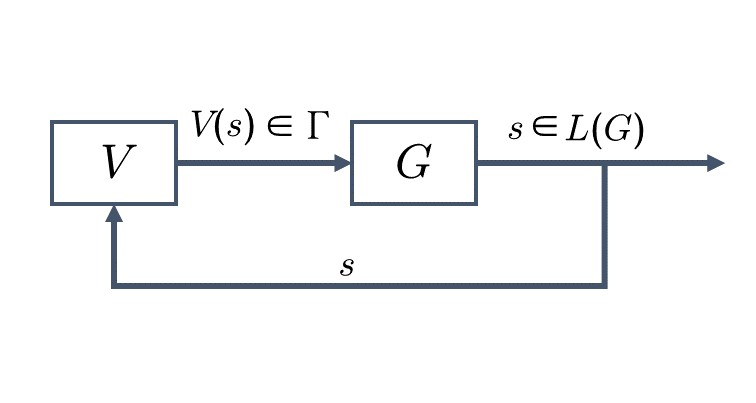
\includegraphics[scale=0.45]{figures/Feedback_Control_Loop.jpg}
    \caption{フィードバック制御ループ}
    \label{fig:Feedback_Control_Loop}
\end{figure}

\begin{enumerate}
    \item $G$は事象列$s \in L(G)$を生成する.
    \item $s$に対して,スーパーバイザ$V$が制御パターン$V(s) \in \Gamma$を生成する.
    \item 次の2つを満たした場合, $G$は$s$に続く$\sigma$を生成する.
    \begin{enumerate}
        \renewcommand{\theenumii}{\roman{enumii}}
        \item $\sigma \in V(s)$($V$に許可された$\sigma$)
        \item $s\sigma \in L(G)$($G$で,$s$の後物理的に起こり得る$\sigma$)
        \end{enumerate}
  \item $s\sigma$を$s$に代入し,$1$へ戻り繰り返す.
\end{enumerate}

$V/G$によって生み出される言語は$L(V/G)$とかき,以下のように定義する.
\begin{enumerate}
    \renewcommand{\labelenumi}{(\roman{enumi})}
    \item $\epsilon \in L(V/G)$
    \item $s \in L(V/G)\ \&\ \sigma \in V(s)\ \&\ s\sigma \in L(G) \Rightarrow s\sigma  \in L(V/G)$
    \item (i),(ii)以外の事象列は$L(V/G)$に属しない.
\end{enumerate}

また$L(V/G)$について三式が成り立つ.

\begin{eqnarray}
    L(V/G)&\neq&\emptyset\\L(V/G)&=&\overline{L(V/G)}\\L(V/G)&\subseteq&L(G)
\end{eqnarray}


\subsection{可制御性}

制御要求を満たす言語$K \subseteq L_m(G)$をおく.$V/G$のマーク言語$L_m(V/G)$を以下のように定義する.
$$L_m(V/G) \coloneqq L(V/G) \cap K$$
また,このときの$V$を$(K, G)$に対するマーキングスーパーバイザ制御と呼ぶ.
$\overline{L_m(V/G)} = L(V/G)$のとき,$V$はノンブロッキングである.そして,$K$が制御可能のときかつその時に限り,ノンブロッキングである$(K,G)$に対する$V$が存在する.制御可能であるというのは,$\overline{K}$に含まれるすべての事象列について
\begin{equation}
    \overline{K}\Sigma_u\cap L(G)\subseteq\overline{K}
\end{equation} 
が成り立つときの$K$をいう.
%言い換えれば制御可能とは,不可制御事象が生起したとしても受理状態まで到達可能であることをいう.%ここがまだ直せてない


制御可能であれば,制御要求を満たすスーパーバイザが存在する.つまりノンブロッキングなマーキングスーパーバイザを作ることができるかどうかは可制御性に依存している.


\subsection{最大許容スーパーバイザ}

$K$の制御可能な部分言語すべての集合を$C(K)$とかく.
\begin{equation}
    C(K)\coloneqq\{K^\prime\subseteq K\mid\overline{K^\prime}\Sigma_u\cap L(G)\subseteq\overline{K^\prime}\}
\end{equation}

また,以下のような式で表せる,$C(K)$の要素のうちすべての$K^\prime$を含んでいる最大要素$supC(K)$を定義する.

\begin{equation}
    supC(K) \coloneqq \bigcup\{K^\prime\mid K^\prime\in C(K)\}
\end{equation}

制御要求の言語$E(E\subseteq\Sigma^\ast)$が与えられて$K=E\cap L_m(G)\subseteq L_m(G)$とし,$K_{sup}=supC(K)$($\neq\emptyset$)であったとする.このとき,
\begin{equation}
    L_m(V_{sup}/G)=K_{sup}
\end{equation}
となる$(K_{sup},G)$に対するノンブロッキングなマーキングスーパーバイザ制御$V_{sup}$が常に存在する.またこのときのスーパーバイザを最大許容スーパーバイザとよぶ.

\clearpage

% 3.
\chapter{Human-in-the-Loopモデリング}

この章では,本研究が着目する倉庫のモデル,およびロボットと人間のエージェントとしての定義をする.また,スーパーバイザの設計方法についても述べる.

\section{倉庫のモデル化}

倉庫の大きさや商品を保管する棚の配置など,倉庫によって構造が異なってくる.本研究では図\ref{fig:Warehouse_gen}のような倉庫を考える.この倉庫の中で複数のロボットと人間がそれぞれの作業をするシナリオを考える.倉庫は,待機場所,通路,棚,搬出場所の4つの要素で構成されている.

上をロボットの待機位置,下をロボットが荷物を届ける搬出場所であると同時に人間が通常作業している場所である。上と下以外の色付きの部分を荷物の保管されている棚として,それら以外は通路とする.この通路はロボット一台が通れるくらいの幅で,すれ違うことは不可能であると想定する.

\begin{figure}[h]
    \centering
    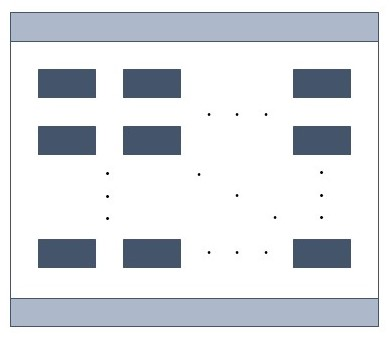
\includegraphics[scale=0.5]{figures/Warehouse_gen.jpg}
    \caption{倉庫の構成}
    \label{fig:Warehouse_gen}
\end{figure}

すべてのロボットにおいて,商品を積み込むときを除いて,いかなるときも棚に侵入できない.そして,棚に侵入するときは必ず上から入り下から出ていく.また,ロボットは前もしくは,右か左に進む動きしかできず,後ろ向きには進めないものとする.

ロボットは上の待機場所でタスクを割り当てられるのを待ち,割り当てられたら目的の品があるところまで行き,商品を積み,下の搬出場所までいく.ここでのタスクを割り当てられるというのは,スタート地点,ゴール地点,商品の場所の3つを与えられることである.スタート地点は待機場所の一段下の状態を,ゴール地点は搬出場所の一段上の状態を指す.商品の場所は棚のうちの一つを指す.

そして人間は、通常下で作業しており,トラブルが発生したときや,人間の協力が必要になったとき,ロボットも通る通路を使って目的の場所まで行く.また,人間はスーパーバイザの制御対象ではない.つまり,人間を制御できない対象として制御システム扱う必要がある.

また,倉庫内で複数台のロボットを制御するとき,以下の点において,注意する必要がある.
\begin{itemize}
    \item 安全性:ロボット同士や人間とロボットの接触(衝突)を防ぐ
    \item デッドロック状態の回避:図のように,お互いのロボットが道を塞いでしまい,動けなくなる状態になることを回避する
    \item 効率性:すべてのロボットが荷物を届け終えるまでの時間が最短になるようにする
\end{itemize}
安全性については,ロボットだけの制御が場合,2台のロボットが同じ状態に存在することを禁止する条件を,すべてのロボットの組み合わせで定めて制御要求として与える.スーパーバイザによってロボットの衝突を回避することが可能になる.
しかし,この制御に人間が加わるとなると,より高度な安全性を考える必要がある.

デッドロック状態は図\ref{fig:Dead_Lock}のようにお互い進めなくなる状況である.これはノンブロッキングであることをスーパーバイザに要求することで解決される.
%あとは効率性の説明

\begin{figure}[h]
    \centering
    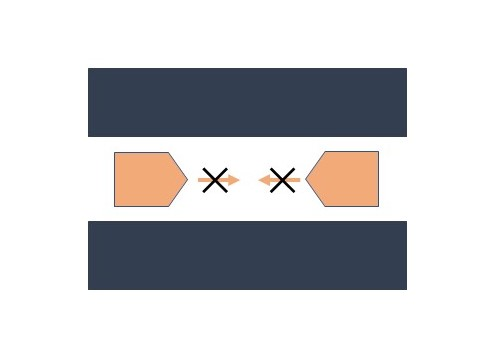
\includegraphics[scale=0.5]{figures/Dead_Lock.jpg}
    \caption{デッドロック状態}
    \label{fig:Dead_Lock}
\end{figure}


\section{ロボットのモデル化}\label{sec:design_robot}

倉庫内のロボットはすべてオートマトンで設計する.第2章で紹介したオートマトンのように5つの要素で構成する$n(>1)$台のロボットを考えるとき,ロボットのオートマトンを以下の$G_i(i=1,2,\ldots,n)$で定義する.
\begin{equation}
    G_i=(Q_i,\Sigma_i,\delta_i,q_{0,i},Q_{m,i})
\end{equation}
ここで$Q_i$は$i$台目のロボットの最短経路上の全状態の集合,$\Sigma_i$は$i$台目のロボットの動作の集合,$\delta_i$は状態遷移関数,$q_{0,i}$は待機場所の状態,$Q_{m,i}$は搬出場所の状態で構成されている.ロボットの動作は表\ref{tb:event_numbers}にあるように設定する.TCTでは奇数の事象が可制御事象,偶数の事象が不可制御事象として処理される.ロボットの動作はすべて可制御事象なので奇数で与える.ここでは北,東,南,西に進むと記載しているが,図で示す場合,それぞれ上,右,下,左で表す.

\begin{table}[htb]
    \centering
    \begin{tabular}{|c|c|} \hline
        事象 & 番号 \\ \hline
        北へ進む & $i\times10+1$ \\
        東へ進む & $i\times10+3$ \\
        南へ進む & $i\times10+5$ \\
        西へ進む & $i\times10+7$ \\ \hline
    \end{tabular}
    \caption{$i$台目のロボットの事象に振られる番号}
    \label{tb:event_numbers}
\end{table}

\section{人間のモデル化}

倉庫内の人間も,ロボットと同様にオートマトンで定義する.人間が$m$人倉庫内に立ち入るとする.ある人間$H_j(j=1,2,\cdots ,m)$の普段の作業場所である一番下の位置(搬出場所)を初期状態$q_{0,H_j}$,戻るべき目的地を$Q_{m,H_j}$,最短経路上の全状態の集合を$\Sigma_{H_j}$状態遷移関数を$\delta_{H_j}$とおいて,人間のオートマトンを以下で表す.

\begin{equation}
H_j=(Q_{H_j},\Sigma_{H_j},\delta_{H_j},q_{0,H_j},Q_{m,H_j})
\end{equation}

人間とロボットが存在する倉庫では,人間の安全面を絶対に確保することが求められ,最優先に考える必要があり,第4章で解説する.


\section{スーパーバイザの設計}\label{sec:design_sup}
スーパーバイザを計算する手順について解説する.

本研究ではTCTという離散事象システムの計算に特化したソフトウェアを使用し,計算を行う.

$N$個の要素(エージェント)と$K$個の制御要求が与えられたとする.

$n$台のロボットの初期状態,受理状態,状態遷移をもとに,それぞれのオートマトン$G_1,G_2,\cdots,G_n$を作成する.また,人間のオートマトン$H_1, H_2, \cdots, H_m$も作成する.$n$と$m$について,$n+m=N$と書くことができる.

%そして,2つのオートマトンの状態のペアを与えて,同時刻に2つのオートマトンそれぞれが与えられた状態のペア存在することを禁止する関数mutexを使用して,制御要求のオートマトン$E_1,E_2,\cdots,E_K$を作成する.
2つのオートマトンに対して,2つの状態で構成される状態のペアを与えられると,オートマトンそれぞれが状態のペアの状態に同時に存在しないようにする関数mutexという関数がある.この関数で出力されるオートマトンを,制御要求のオートマトン$E_1,E_2,\cdots,E_K$とする.

次に,$G_1,\cdots,G_n,H_1,\cdots,H_m$のすべてのオートマトンを同期合成させ,制御対象であるPLANTを出力する.このとき,受理状態のみ存在し,PLANTのすべての事象で自己ループする遷移が定義されるオートマトンALLを作成する.

$E_1$から$E_K$までのすべての制御要求とPLANTの全事象を含んだALLを同期合成させ,制御要求SPECを生成する.

Supconと呼ばれる関数にPLANTとSPECを入力し,制御要求を満たすスーパーバイザを得る.


\clearpage

% 4.
%人間はロボットと同じ速度で動く


%本研究では,スーパーバイザの計算結果から,最適なふるまいを選び出す.
%全エージェントを同時に動いたとする.
%人間の安全を保障するため,最後に人間の行動を決定する.
%

\chapter{Human-in-the-loopにおける人間の安全性を確保する方法}\label{chap:method}

この章では,人間を考えた倉庫の中で人間の安全性を確保するためにどう制御するかという問題に対しての2つの方法を提案する.人間の普段の作業場所をスタート地点といい,トラブルが発生した場所,もしくはロボットに協力するために向かうロボットとの合流地点を目的地,そして人間が最終的に戻りたい場所をゴール地点とよぶこととする.
% トラブルなどを処理し終わった人間がそれまで行っていた作業に戻る場合,スタート地点とゴール地点が同じ地点になる.

\section{方法1}
1つ目の方法は,人間が使う通路上(スタート地点から目的地に向かうまでの経路と目的地からゴール地点に向かうまでの経路)をロボットに使わせないという考え方で制御を行う.人間が通る可能性のある通路についてロボットを完全に通行止めにする(図\ref{fig:area}).図の赤い部分がロボットの進入禁止エリアである.

\begin{figure}[h]
    \centering
    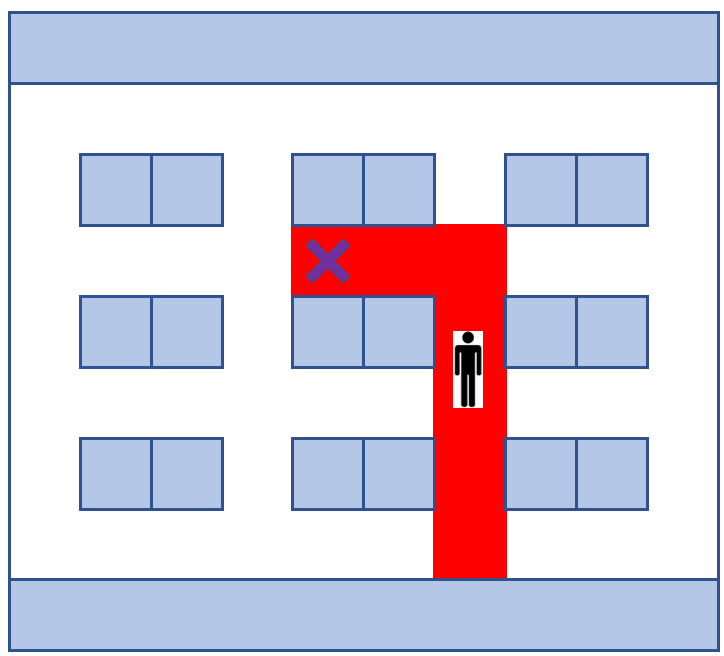
\includegraphics[scale=0.3]{figures/4_area.png}
    \caption{ロボットの進入禁止エリア}
    \label{fig:area}
\end{figure}

これを実現する具体的な方法は,不可制御事象をもちいて人間の行動を定義する方法である.行動すべてを不可制御事象で定義するということは,スーパーバイザからみて,人間の行動がいつ発生するかわからない,かつ発生を禁止することができない. 
\ref{sec:design_robot}節のとおり,倉庫内を移動しているロボットはスーパーバイザ制御理論でいう可制御事象で定義されており,指示を出すことができる制御対象である.それに対して人間は制御対象ではない.

例えば,ロボットに対しては「特定の場所で方向転換し,あるタイミングで,決まった速度で移動する」というように精密に指示することが可能だが,人間はロボットのように厳密に制御できるわけではなく,本人の意思によっても行動する.したがって,人間を制御するのではなく,制御対象ではないとするのが自然である.

ロボット同士の制御であれば,制御要求を満たさない行動,つまり衝突してしまう行動やブロッキング状態になってしまう行動を直前で禁止することができた.しかし,不可制御事象で定義された人間に対しては,スーパーバイザは制御要求を満たさない行動を禁止できない.また,人間の行動のタイミングもコントロールするのが不可能である.ロボットが人間の経路上に存在していると,連続して何回も人間が行動し続けた場合,衝突することになり制御要求を満たさない.このような理由で人間の経路はロボットから見て障害物のように認識される.
これを踏まえて,スーパーバイザが計算される.

この計算結果として,人間が安全な場所に到着するまで,人間の経路上にロボットを侵入させないというスーパーバイザが得られる.

% なんか書く.スーパーバイザ作る具体的な手順とか?

言い換えれば,人間のスタート地点から,トラブルが発生した場所や協力が必要なロボットとの合流地点までの経路を予約し,予約された通路をロボットから見て通行止めとすることで,人間の経路上には完全に立ち入らせず安全を確保する方法である.


\section{方法2}
2つ目の方法は,人間のいる位置を重視して,人間の周りだけにロボットの進入禁止エリアを定めるというものである.
1つ目の方法は,ロボットの進入禁止エリアを静的に定めていたのに対し,2つ目の方法では動的に変化する.

衝突回避の制御について,ロボット同士の場合は,どちらかのロボットの進行方向に別のロボットがいるときに行動を禁止している.これが人間とロボットの場合,人間の前に来てからロボットの行動を禁止するのでは,人間の恐怖心をあおるだけでなく,万が一エラーが起こることも考慮に入れると事故のもとになるという理由から,ロボットと人間の間に一定の距離を設ける必要性がある. 

また,そのロボットと人間が安全を確保するために最低限離れていなければならない距離(最小安全隔離距離)を任意に決められるように変数で扱うことにより汎用性を高める.ロボットの移動速度が大きければ制動距離のことを考慮して最小安全隔離距離を大きくとり,逆に移動速度が小さければ最小安全隔離距離も小さくするというように,最小安全隔離距離を変数とし,変更可能にすることにより様々なスペックのロボットに対応することができる.また,倉庫の規模によって変更することもできる.

具体的な方法としては,制御要求を拡張することで実現する.ロボットだけを制御するとき,制御要求は衝突回避のため,同じ瞬間に同じ位置に2つ以上のエージェントが存在する状態を排斥していた.それに対し提案する方法では,最小安全隔離距離を1マスとおいた場合,図\ref{fig:d=1}のように制御要求を人間を中心としてロボットが前後左右のマスにいる状態にまで拡張させる.また,最小安全隔離距離を2,3とおいた場合,それぞれ図\ref{fig:d=2},\ref{fig:d=3}のように進入禁止エリアを設定する.基本的に,ロボットが通路もしくは棚にいるときに接近を禁止する.ロボットが倉庫の待機場所もしくは搬出場所にいるときは距離をとる必要がないので進入禁止エリアに指定していない.

%この方法を使った場合,人間がすぐにはたどり着かない場所,つまり人間の安全が十分に確保されている場所はロボットも通ることができる.

\begin{figure}[h]
    \centering
    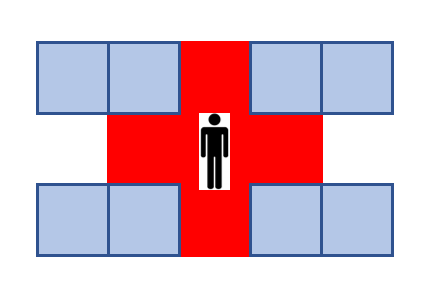
\includegraphics[scale=0.5]{figures/4_d=1.png}
    \caption{最小安全隔離距離 $d=1$}
    \label{fig:d=1}
\end{figure}

\begin{figure}[h]
    \centering
    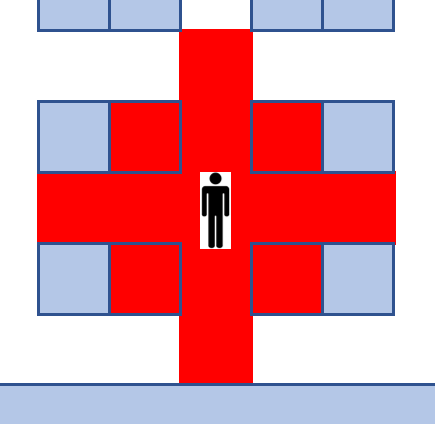
\includegraphics[scale=0.5]{figures/4_d=2.png}
    \caption{最小安全隔離距離 $d=2$}
    \label{fig:d=2}
\end{figure}

\begin{figure}[h]
    \centering
    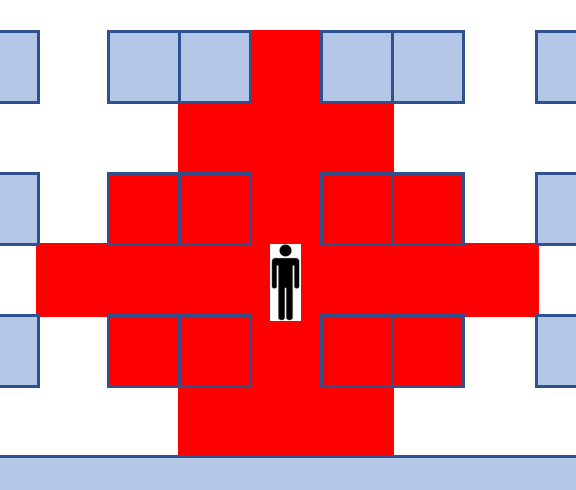
\includegraphics[scale=0.5]{figures/4_d=3.png}
    \caption{最小安全隔離距離 $d=3$}
    \label{fig:d=3}
\end{figure}


\ref{sec:design_sup}節の手順で計算を行うと,ロボットと人間がとり得るデータで制御要求を満たす状態遷移のすべてを網羅したスーパーバイザが出力される.そのスーパーバイザの状態遷移のうち,初期状態からどのようなふるまいで受理状態までの到達するのか選択する必要がある.すべてのエージェントが1回行動するもしくは行動しない一連の事象列の経過を単位時間(スーパーバイザの対象の数が$x$とすると\ $単位時間<x遷移$)とする.ロボットのみの制御を行う場合,スーパーバイザの初期状態から受理状態までかかる時間が最小のものを選ぶことで最も効率の良いタスクの処理といえる.しかし,人間を含めた制御を行う場合,たとえタスクを完了させるまでの時間が短くても,安全性を考えると人間の行動を禁止してロボットを優先する制御をすべきではない. 

また,実用化する観点からみたとき,ロボットのコストと人間のコストを比べると,ロボットを導入して運用することについては,運用費に対する初期投資が大きく,人を雇用するのについては,雇う時間が長ければ長いほどコストがかかると推測される.つまり,ロボットは固定費,人間は変動費といったように大まかに考えることにする.人件費においてはコスト削減の余地があるという点においても,ロボットと人間どちらかの行動を禁止するとなったとき,人間の行動を優先して,倉庫内の移動時間を短くすることが重要である.



\clearpage

% 5.
\chapter{倉庫でHuman-in-the-loopした場合のシミュレーション検証}

第\ref{chap:method}章で紹介した2通りの方法を用いて,人間が必要とされる具体的な事例をいくつか想定し,それらの方法を用いて問題解決できることを示す.2台のロボットと1人の人間についてスーパーバイザ制御を行い,計算されたスーパーバイザをもとにシミュレーションを作成する.ロボット1とロボット2のオートマトンをそれぞれ$G_1,G_2$とかき,人間のオートマトンを$H$とかく.

\section{ケース1:棚から商品が落下した場合} \label{sect:case1}
%本研究では,スーパーバイザの計算結果から,最適なふるまいを選び出す.
%全エージェントを同時に動いたとする.
%人間の安全を保障するため,最後に人間の行動を決定する.
%

1つ目のケースでは,人間の臨機応変な対処ができる能力を駆使し,発生の予測が不可能かつ早急に措置しなければならないトラブルに対処することが目的である.

まず,商品が棚から落ちた図\ref{fig:HITL1_case1}のような場合を初期状態と考える.2台のロボットの初期状態は計算上,0としているが,ロボット1($blue$)は状態7の上に,ロボット2($green$)は状態8の上に,一方人間の初期状態である通常作業場所は状態67の下に位置している.またそれぞれのタスクについて,ロボット1は状態33(棚)に,ロボット2は状態36(棚)に,人間はトラブルの発生した場所である状態26(通路上)に設定する.搬出場所については計算上71とするが,$G_1$は状態68の下に,$G_2$は状態65の下に,人間$H$はもとの作業場所であった状態67の下に戻ることとする.

\begin{figure}[t]
    \centering
    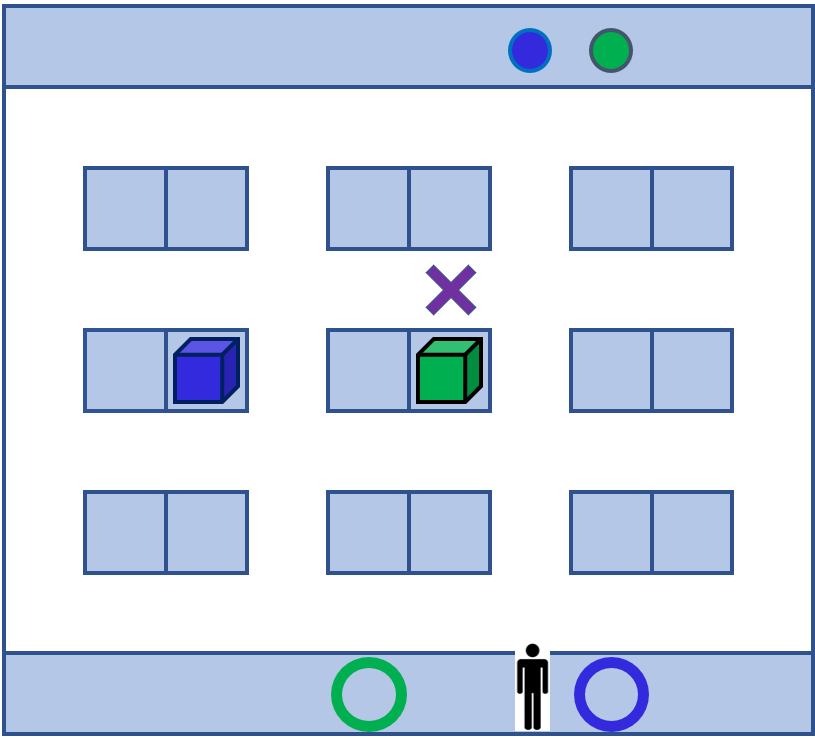
\includegraphics[scale=0.25]{figures/HITL1_case1.png}
    \caption{初期状態(ケース1)}
    \label{fig:HITL1_case1}
\end{figure}

ケース1では,人間は棚から落ちた商品をもとあった収納スペースに返し,すぐ元の作業場所へ戻ってくると想定する.

ロボットのオートマトン$G_1$,$G_2$と人間のオートマトン$H$の遷移関数はそれぞれの最短経路のみで定義するので,経路はそれぞれ図\ref{fig:HITL1_case1_G1},\ref{fig:HITL1_case1_G2},\ref{fig:HITL1_case1_H}とする.

\begin{figure}[b]
    \centering
    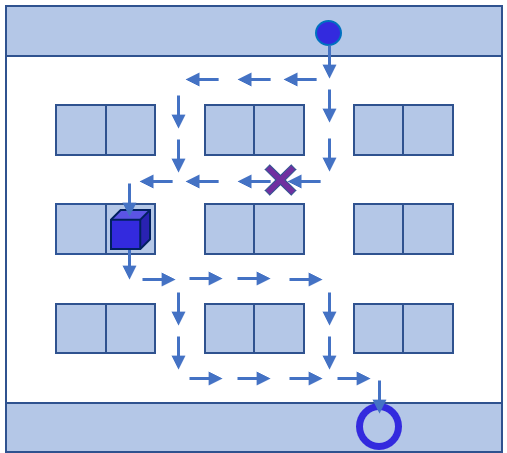
\includegraphics[scale=0.38]{figures/HITL1_case1_G1.png}
    \caption{ロボット1の経路(ケース1)}
    \label{fig:HITL1_case1_G1}
\end{figure}
\begin{figure}[!t]
    \centering
    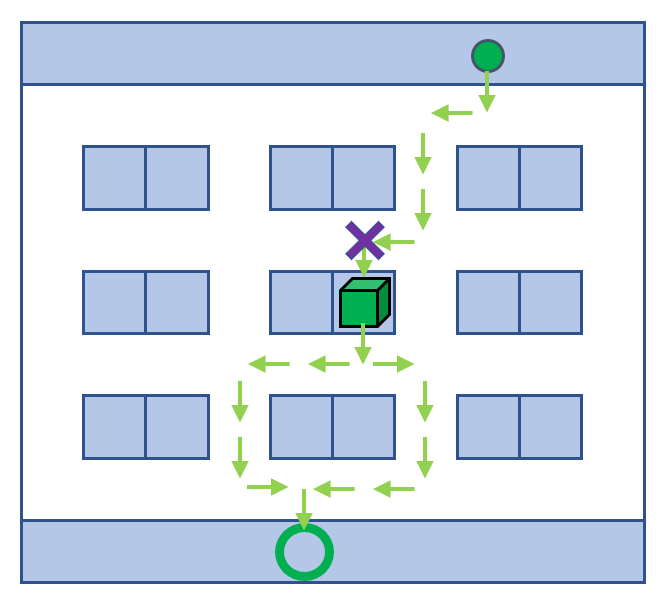
\includegraphics[scale=0.3]{figures/HITL1_case1_G2.png}
    \caption{ロボット2の経路(ケース1)}
    \label{fig:HITL1_case1_G2}
\end{figure}
\begin{figure}[!t]
    \centering
    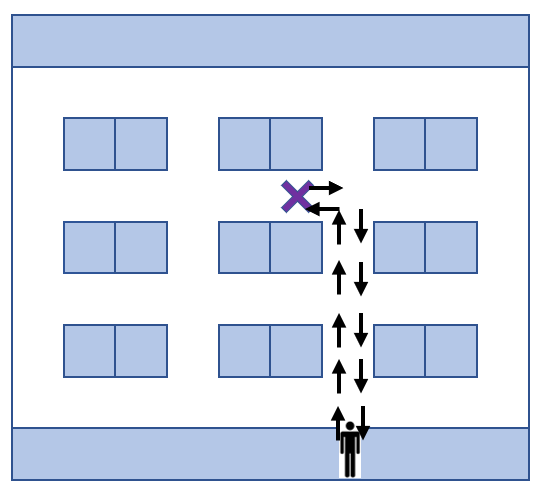
\includegraphics[scale=0.35]{figures/HITL1_case1_H.png}
    \caption{人間の経路(ケース1)}
    \label{fig:HITL1_case1_H}
\end{figure}

落ちた商品で通路を塞いでしまうのでそのことに関しても考慮しなければならない.

このケースは,ロボット1ではトラブルの発生場所である状態26を通る経路がいくつかある最短経路のうちの1つとなっている.ロボット1に関して言えば,落下した商品で通路が使用できなくなっている経路を削除しても支障はない.しかし,ロボット2のオートマトン$G_2$のようにトラブルの発生場所を使う経路しか定義されていないとき,そもそも受理状態まで到達できないという問題点が挙げられる.また,仮に搬出場所付近でこのトラブルが発生したとき,トラブルが処理されてすでに通ることができるにもかかわらず経路を削除してしまい効率の良いふるまいを見逃す可能性もある.
落下した商品に関するオートマトンを作成し,それをもちいて制御要求を定めることで,これらの問題を解決する.

%通路に落ちた商品で経路を塞いでしまう問題を解決する.
商品に関するオートマトン$O$は通路に落ちている状態0と棚に収納されている状態1の2つの状態で構成されるオートマトンで,初期状態を0,受理状態を1とする(図\ref{fig:automatonO}).状態遷移は人間がトラブルを処理する事象(人間と共通の事象)が発生したとき,0から1に移る状態遷移のみ定義する.ここで,指定した状態の組を排除するmutexという関数をもちいて制御要求を定める.

$G_1$と$O$,$G_2$と$O$について,mutexを使用し,状態の組み合わせ$P_{O,G_i}=[0,26]$を取り除く制御要求を与える. $P_{O,G_i}$の1つ目の要素は$O$の状態,2つ目の要素は$G_i$の状態を示している.こうしてロボットの状態とトラブルが処理できていない状態の組み合わせを除くことで,商品が通路上にあるとき塞がった通路の使用を禁止し,かつ商品が棚に戻されたあとは通路の使用を許可する制御要求を与える. 

\begin{figure}[t]
    \centering
    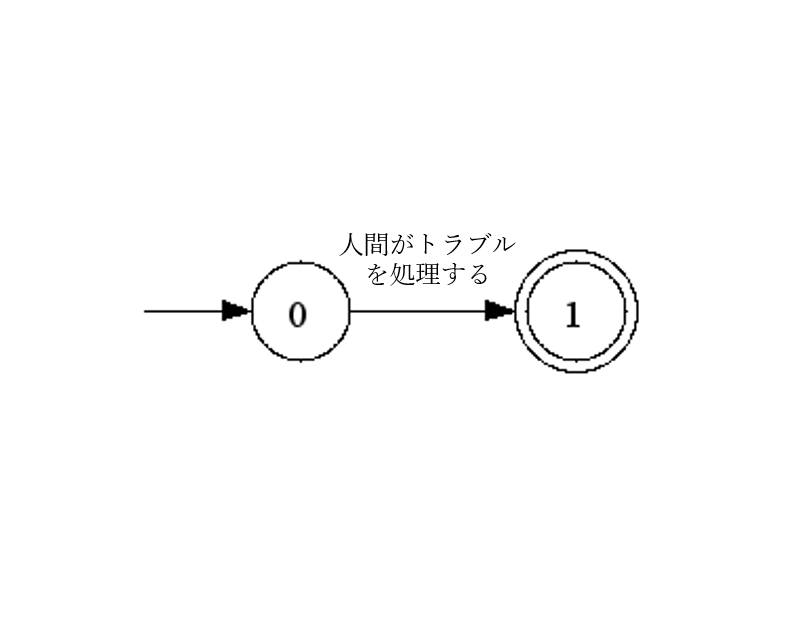
\includegraphics[scale=0.4]{figures/automatonO.png}
    \caption{落下した商品についてのオートマトン}
    \label{fig:automatonO}
\end{figure}

$H$の状態遷移の定義について,スタート地点からトラブルが発生した場所へ向かう遷移と,その逆にトラブルの場所からもといた場所へ戻ってくる遷移があり,方法1では,これらはすべて不可制御事象によって遷移する.極端な話,1マス進んで1マス戻るという遷移で受理状態に到達する可能性もあるが,スーパーバイザは行動を禁止することができずこれに対して対処できない.トラブルの発生場所を通る経路しか定義されていないロボットが含まれていた場合,人間のトラブル処理の事象が起こるまで受理状態にいくことはない.しかし,先ほどの1マス進んで1マス戻る例では,人間がトラブルを処理せず受理状態に到達する可能性があるため,条件を満たすスーパーバイザが存在しないことになる.

\begin{figure}[!t]
    \centering
    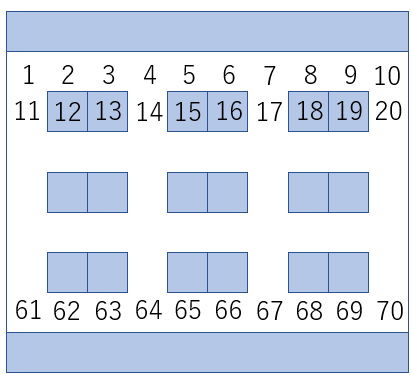
\includegraphics[scale=0.5]{figures/Warehouse_before.png}
    \caption{トラブルの処理前の状態に割り当てる番号}
    \label{fig:Warehouse_before}
\end{figure}
\begin{figure}[!t]
    \centering
    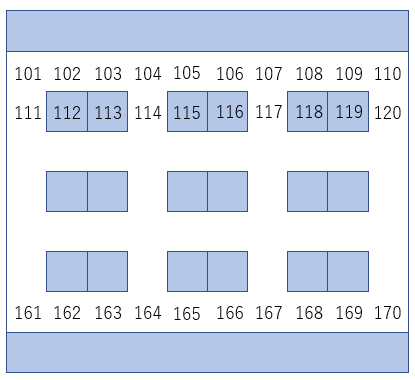
\includegraphics[scale=0.5]{figures/Warehouse_after.png}
    \caption{トラブルの処理後に状態に割り当てる番号}
    \label{fig:Warehouse_after}
\end{figure}

人間の遷移が可制御事象で定義されていれば,オートマトン$O$を制御要求にすることにより,人間がトラブルを処理する前に受理状態に到達することがないように設定が可能だ.しかし,人間の行動を不可制御事象にしてこの制御要求を与えても,条件を満たすスーパーバイザは存在しない.

これを解決するため,行きの状態と帰りの状態を区別することで,トラブルを処理する前に途中で引き返して受理状態にたどり着かないように設計した.状態の番号を図\ref{fig:Warehouse_before},\ref{fig:Warehouse_after}のように割り当てる.トラブルを処理する事象が起これば,帰り用の状態に遷移する.

商品で通路が塞がれているときはその場所を通る経路を削除し,人間がトラブルを処理したのち,削除した経路を追加しスーパーバイザの再計算を行うという方法も考えたが,現時点ではオンライン制御を実現できておらず,今後の課題として検討する.

\subsection{方法1} \label{sec:case1_method1}
方法1の場合,人間の行動を表\ref{tb:event_numbers_human1}のように定義することで,人間の経路はロボットからみてすべて通行不可となる方法であった.ここで,北,東,南,西に進む事象は,図で示すとそれぞれ上,右,下,左に進むことを意味する.トラブルを処理する事象は状態$s$に存在したとすると,状態$s$から状態$s+100$に遷移するという事象である.ロボットの進入禁止エリアは図\ref{fig:human_area}のように表され,人間が通る可能性がある限りロボットは進入できない.

\begin{table}[htb]
    \centering
    \begin{tabular}{|c|c|} \hline
        事象 & 番号 \\ \hline
        北へ進む & $100$ \\
        東へ進む & $102$ \\
        南へ進む & $104$ \\
        西へ進む & $106$ \\ 
        トラブルを処理する & $108$ \\ \hline
    \end{tabular}
    \caption{$H$の事象に振られる番号(ケース1,方法1)}
    \label{tb:event_numbers_human1}
\end{table}

\begin{figure}[!t]
    \centering
    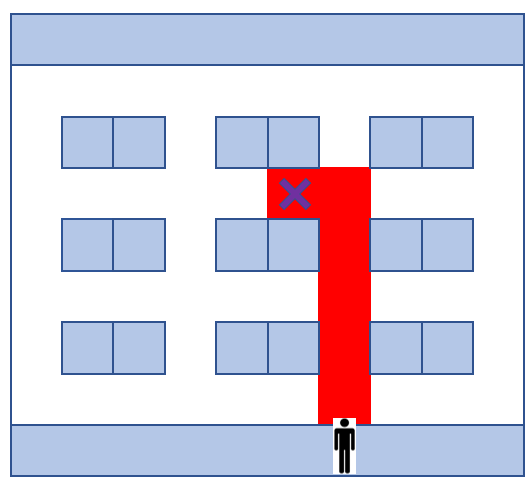
\includegraphics[scale=0.3]{figures/5_human_area.png}
    \caption{ロボットの進入禁止エリア(ケース1,方法1)}
    \label{fig:human_area}
\end{figure}

行きと帰りの状態を分けることで起こってしまう問題がある.それは,トラブルを処理した後で,人間が通り過ぎたところからロボットが通路として使用するのが許可されることだ.作業場所に戻っている最中の人間のすぐ後ろをロボットが追尾する行動を許してしまうことになる.これでは,十分に安全ということはできない.

ここで新しいオートマトン$P$を定義する.図\ref{fig:automatonO}のオートマトンのように,状態が2つ,遷移関数は初期状態から受理状態に遷移する事象ただ1つのみで定義する.$H$が受理状態にいるときに自己ループする事象を定義し,その事象と$P$の唯一の事象を一致させることによって,$H$が受理状態に到達した後で,$P$は状態0から状態1に遷移することになる.

そして,mutexを使用し,$P$が状態0に,$G_1,G_2$が人間の経路上の状態に存在する組み合わせを排除する.
これを制御要求に追加することで人間がもともといた作業場所に戻るまで,人間の経路に侵入するロボットの行動を禁止し続けることが可能である.
オートマトン$P$は,人間が搬出場所に戻ったときのみ作動する,人間の安全を確認するスイッチのような働きをする.

$G_1,G_2$と$H$について,衝突が起こらないようにそれぞれが同じ状態にいる状態を$PLANT$から除く要求と,通路に落ちた商品が棚に戻されるまで,落ちた商品の位置にいる状態を除く要求を制御要求として与える.これらの制御要求をもとにスーパーバイザを作成し,フィードバックループ制御システムを構成する.

スーパーバイザによってどのような制御アクションを行われるかシミュレーションで解説する.

図\ref{fig:HITL1_case1_a}のような状態を状態$a$と呼ぶことにする.状態$a$のときロボット1は状態7に位置しており,ロボット2は状態8に位置している.このとき,次に生起するロボットの行動の選択肢として,$G_1$が行動15によって状態17へ遷移,$G_1$が行動17によって状態6へ遷移,$G_2$が行動27により状態7へ遷移する3つが存在する.
ここでロボット2が行動17で左に移動してしまった場合はロボット1と衝突することになり,制御要求を満たさない.そのため,このときスーパーバイザは$G_2$の行動27を禁止する.このとき,その他の遷移はスーパーバイザに制御されることなく生起が許可されている.

\begin{figure}[!t]
    \centering
    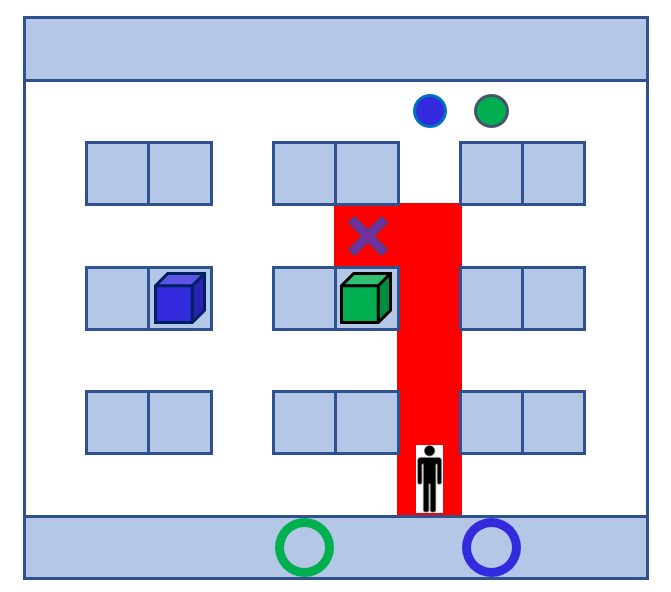
\includegraphics[scale=0.3]{figures/HITL1_case1_a.png}
    \caption{ケース1\ 状態$a$}
    \label{fig:HITL1_case1_a}
\end{figure}

\begin{figure}[!t]
    \centering
    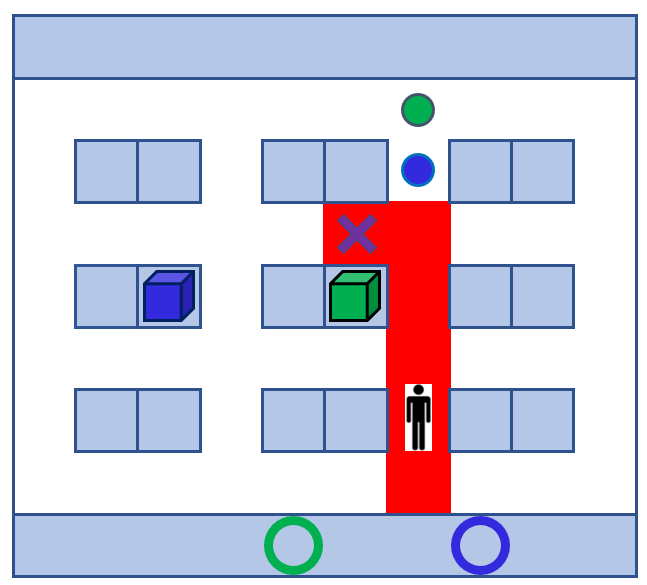
\includegraphics[scale=0.3]{figures/HITL1_case1_b.png}
    \caption{ケース1\ 状態$b$}
    \label{fig:HITL1_case1_b}
\end{figure}

$G_1$は行動15を許可されているので,状態17に進み,その他のエージェント達も遷移して状態$a$から状態$b$(図\ref{fig:HITL1_case1_b})になったと仮定する.このとき状態17からの$G_1$の遷移は行動15により状態27へ移る遷移だけである.しかし,状態27は人間の経路上に指定されているので,スーパーバイザが$G_1$のこの行動を禁止する.人間がトラブルを処理してもとの作業場所に戻るまで,つまり$H$が状態167($G_1$から見ると状態67)から受理状態に遷移して,受理状態での自己ループ事象が生起されるまで,$G_1$の次の行動が禁止され続けることになる.

\begin{figure}[!t]
    \centering
    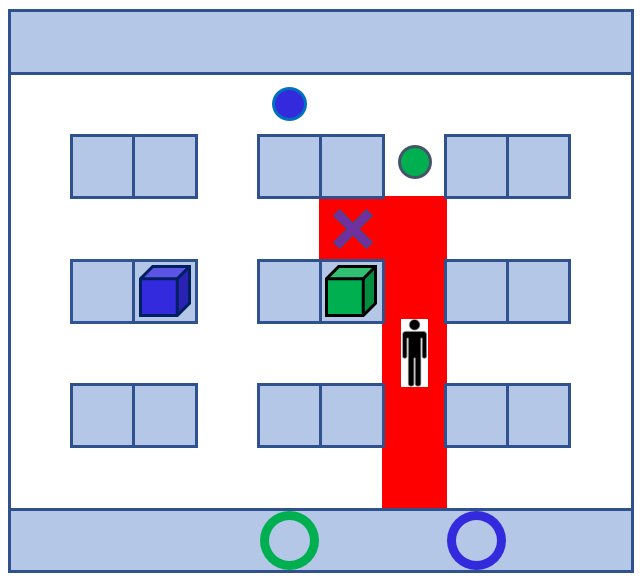
\includegraphics[scale=0.3]{figures/HITL1_case1_c.png}
    \caption{ケース1\ 状態$c$}
    \label{fig:HITL1_case1_c}
\end{figure}

\begin{figure}[!t]
    \centering
    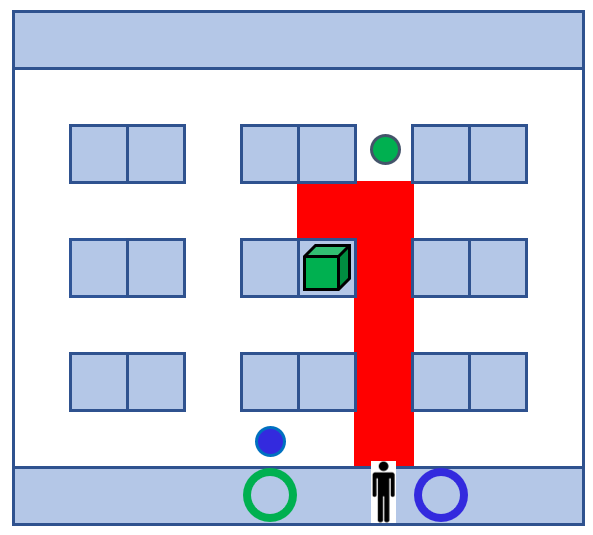
\includegraphics[scale=0.32]{figures/HITL1_case1_d.png}
    \caption{ケース1\ 状態$d$}
    \label{fig:HITL1_case1_d}
\end{figure}

また,状態$a$から,$G_1$が行動17,$G_2$が行動25,$H$が行動100が生起したときの状態を状態$c$(図\ref{fig:HITL1_case1_c})とする.このときも状態$b$のとき同様に,状態17にいる$G_2$の遷移は行動25だけで,行動25により遷移した場合,人間の使用する通路に入ってしまう.制御要求を満たさないので,$H$が受理状態である171で自己ループするまで$G_2$の行動25が禁止される.

%人間がトラブルを処理したのち図\ref{fig:HITL1_case1_d} のように人間が状態37に遷移すると,状態27に人間の通る可能性がなくなり,行動25がスーパーバイザによって許可される.
$H$が受理状態171で安全が確保されたのち,図\ref{fig:HITL1_case1_d}のようにロボットの進入禁止エリアが解除され,対象がロボットだけの自動化制御が行われる.

\begin{figure}[!t]
    \centering
    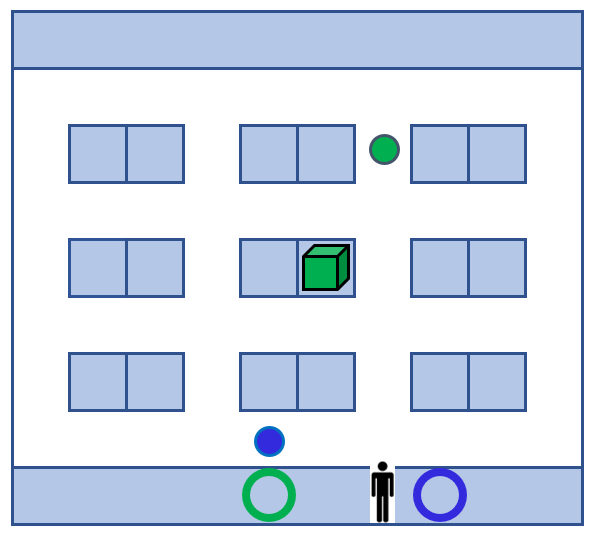
\includegraphics[scale=0.32]{figures/HITL1_case1_e.png}
    \caption{ケース1\ 状態$e$}
    \label{fig:HITL1_case1_e}
\end{figure}



\subsection{方法2}
次に先ほどと同じ例を用いて,方法2によって制御した場合のスーパーバイザについて解説する.

まず,人間の行動を表\ref{tb:event_numbers_human2}のように可制御事象で定義する.

\begin{table}[htb]
    \centering
    \begin{tabular}{|c|c|} \hline
        事象 & 番号 \\ \hline
        北へ進む & $101$ \\
        東へ進む & $103$ \\
        南へ進む & $105$ \\
        西へ進む & $107$ \\ 
        トラブルを処理する & $109$ \\ \hline
    \end{tabular}
    \caption{$H$の事象に振られる番号(ケース1,方法2)}
    \label{tb:event_numbers_human2}
\end{table}

\begin{figure}[!t]
    \centering
    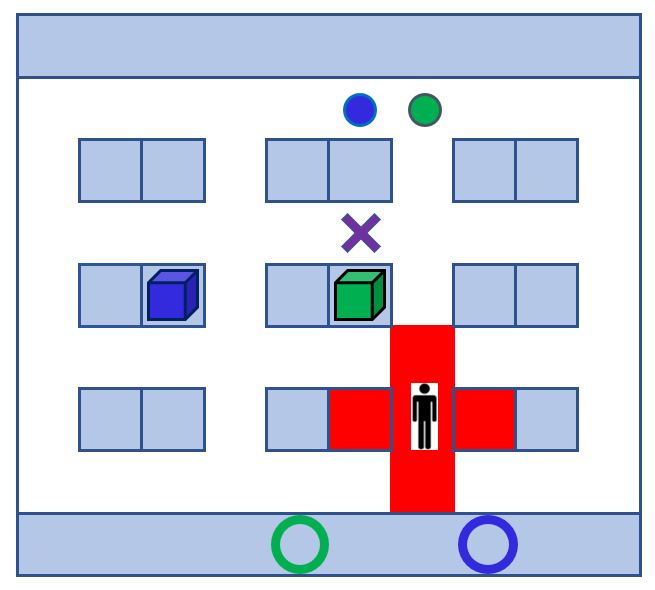
\includegraphics[scale=0.3]{figures/HITL2_case1_f.png}
    \caption{ケース1\ 状態$f$}
    \label{fig:HITL2_case1_f}
\end{figure}

\begin{figure}[!t]
    \centering
    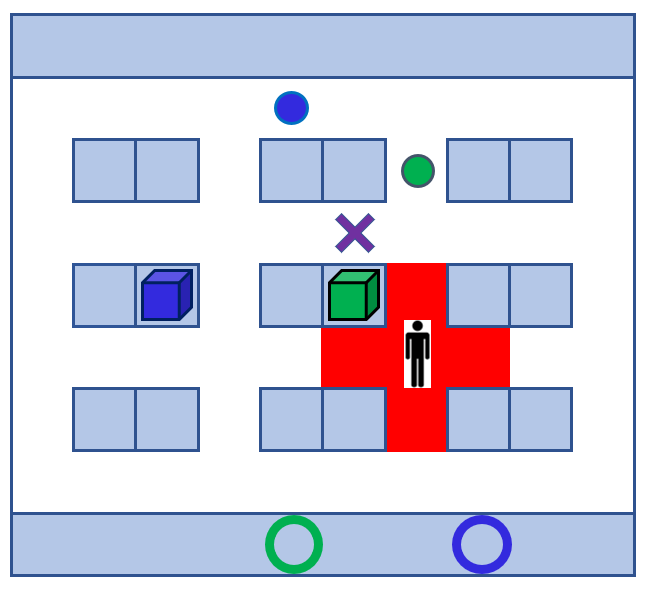
\includegraphics[scale=0.3]{figures/HITL2_case1_g.png}
    \caption{ケース1\ 状態$g$}
    \label{fig:HITL2_case1_g}
\end{figure}

状態$f$(図\ref{fig:HITL2_case1_f})のとき,ロボット2のとり得る遷移は行動25である.しかし,このとき行動25により,状態17に遷移してその他のエージェントも遷移したとき,状態$g$(図\ref{fig:HITL2_case1_g})になる.商品を棚に戻す作業をしない限り,ロボットは状態26に遷移できない制御要求があるのでロボット2は状態27に遷移したとしても受理状態まで到達することはない.また,人間とロボットの間に1マス以上間隔を開けなければいけない制御要求が与えられているため人間は状態27に遷移することができない.この結果,ロボット2と人間はお互い遷移ができないブロッキング状態に陥る.これを防ぐため,スーパーバイザは,状態$f$で,$G_2$の行動25を禁止する.

\begin{figure}[h]
    \centering
    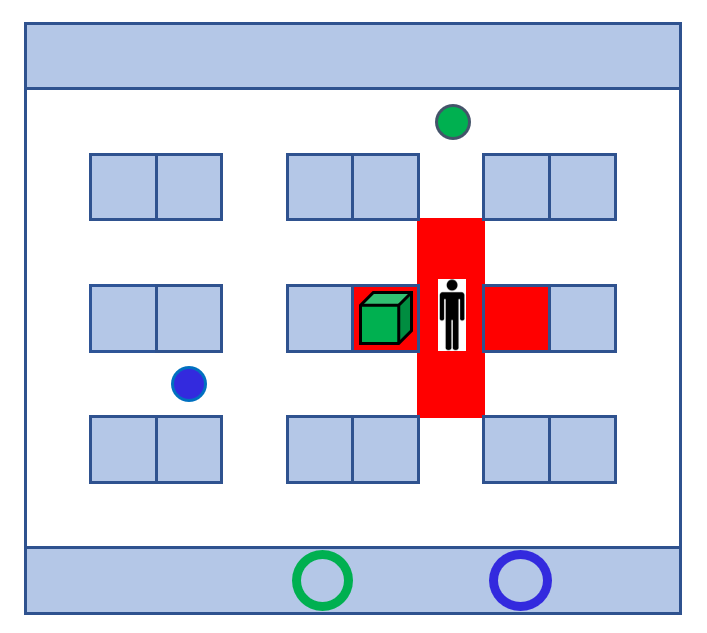
\includegraphics[scale=0.3]{figures/HITL2_case1_h.png}
    \caption{ケース1\ 状態$h$}
    \label{fig:HITL2_case1_h}
\end{figure}

$H$が状態137に遷移した後(図\ref{fig:HITL2_case1_h}),$G_2$の状態7での行動25が許される.


\section{ケース2:人間とロボットが協調する}
% ケース4では,ロボットが荷物を積み込むときに人間の助けが必要な場合
% d=1でいい理由も書く??

段ボール箱単体や,段ボール箱が乗ったパレットを運搬するような単純作業を行う場合,ロボットは能力を発揮する.それに比べて,商品のピッキング作業は不得意であり,今のピッキング技術では,商品の条件に変化があるような複数のタスクを1つのロボットで担うのは,困難であり,近い将来実現するのは難しいと考えられる.また人間は,ピッキング作業を得意としており,小さい品や,柔らかいもの,つぶれやすいものなど,さまざまな商品の条件に対応することができる.

荷物の運搬において,迅速に,かつ一度で大量に運ぶことも可能なロボットと,ピッキング作業において能力を発揮できる人間のそれぞれの長所を生かすことを目的として考えられた事例の制御システムを設計する.

ケース2では,具体的な例として図\ref{fig:HITL1_case2}を考え,ロボットだけでは完遂できない特殊なタスクが状態32(棚)にあり,ロボット1に与えるとする.状態4の上をスタート地点とし,状態64の下に位置する搬出場所へ届けるというタスクが割り当てられている場合を想定する.また,ロボット2にはスタート地点を状態6の上に,搬出場所を状態68の下に,ピックする商品が状態33(棚)にあるタスクを与える.
人間は普段の作業場所を状態66の下とおいて,状態31(通路上)に向かい,ロボット1の手助けをする.このときの人間のポジションを協調作業場所と呼ぶことにする.ケース1と同様に,初期状態と受理状態を普段の作業場とする.

\begin{figure}[!t]
    \centering
    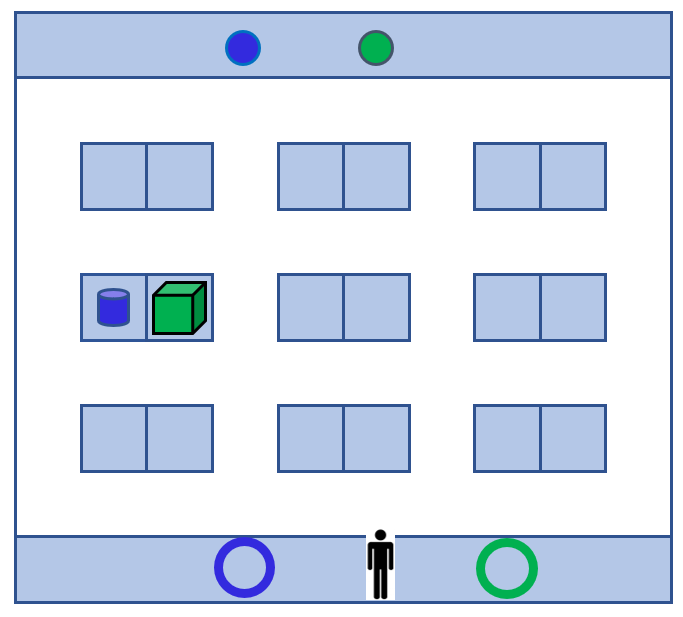
\includegraphics[scale=0.3]{figures/HITL1_case2.png}
    \caption{ケース2\ 初期状態}
    \label{fig:HITL1_case2}
\end{figure}

それぞれの最短経路は図\ref{fig:HITL1_case2_G1},\ref{fig:HITL1_case2_G2},\ref{fig:HITL1_case2_H}になる.

\begin{figure}[!t]
    \centering
    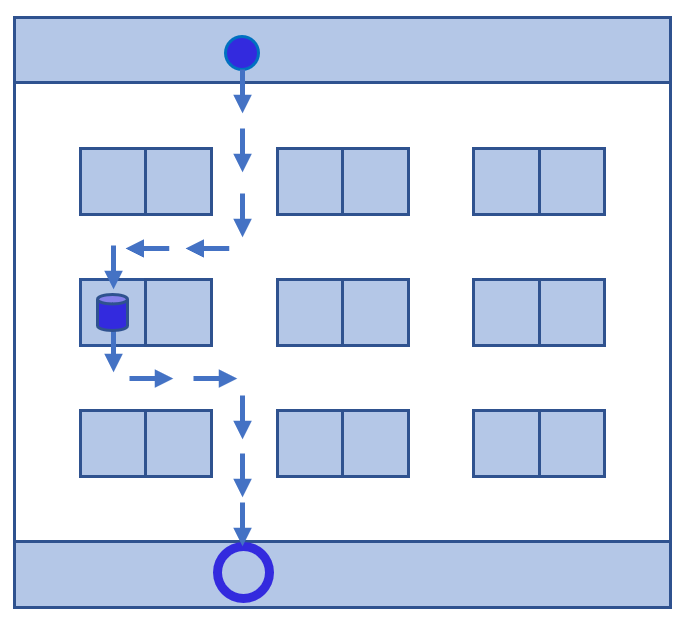
\includegraphics[scale=0.3]{figures/HITL1_case2_G1.png}
    \caption{ロボット1の経路(ケース2)}
    \label{fig:HITL1_case2_G1}
\end{figure}
\begin{figure}[!t]
    \centering
    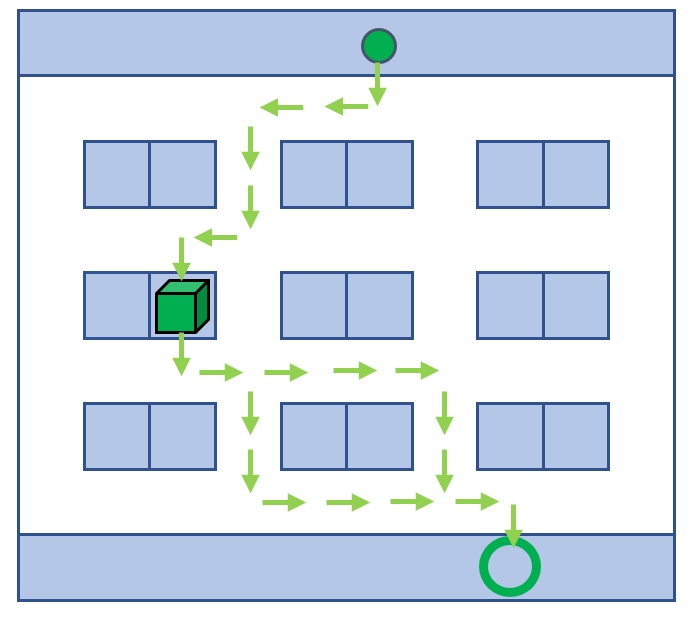
\includegraphics[scale=0.3]{figures/HITL1_case2_G2.png}
    \caption{ロボット2の経路(ケース2)}
    \label{fig:HITL1_case2_G2}
\end{figure}
\begin{figure}[!t]
    \centering
    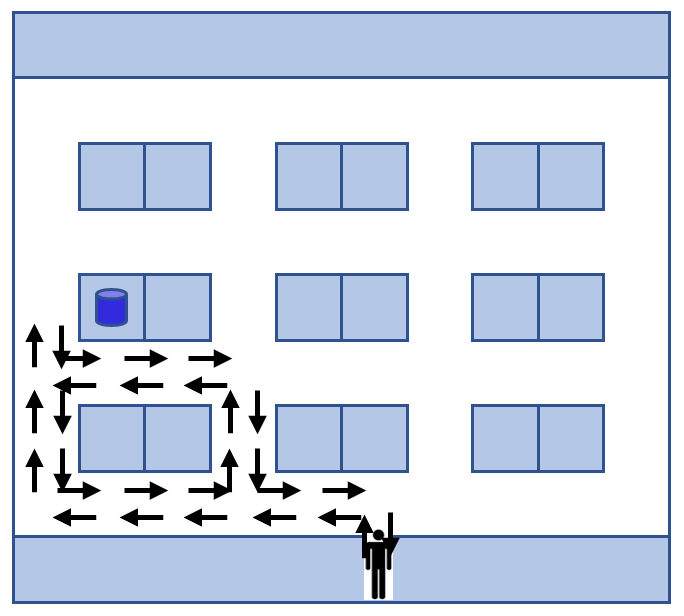
\includegraphics[scale=0.3]{figures/HITL1_case2_H.png}
    \caption{人間の経路(ケース2)}
    \label{fig:HITL1_case2_H}
\end{figure}

またケース1と同様に,図\ref{fig:Warehouse_before},\ref{fig:Warehouse_after}のように行きの状態と帰りの状態を分ける必要がある.


\subsection{方法1}
まず,人間の事象を表\ref{tb:event_numbers_human3}のように設定し,オートマトン$H$を作成する.またロボットの進入禁止エリアは図\ref{fig:human_area_2}となる.

\begin{figure}[!t]
    \centering
    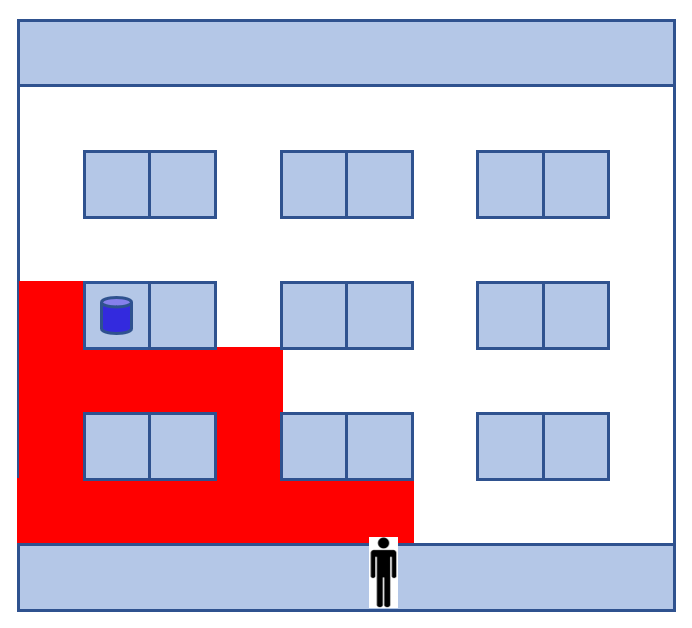
\includegraphics[scale=0.3]{figures/human_area_2.png}
    \caption{ロボットの進入禁止エリア(ケース2,方法1)}
    \label{fig:human_area_2}
\end{figure}

ロボット1は人間の手助けがないとタスクを完了できない.人間が状態31に,ロボット1が状態32に存在しているときのみ協調作業が可能である.人間が到着する前にロボット1が状態32から遷移することや,その逆にロボット1が到着する前に人間が状態31から遷移することを防ぐために,$G_1$に$H$と共通の事象をおく(表\ref{tb:event_numbers_G1}).この事象が生起すると$G_1$は状態32で自己ループし,$H$は状態31から状態131に遷移する.

また,ケース1の方法1(\ref{sec:case1_method1}節)と同様に,$H$の受理状態で自己ループを行う事象を定義する.その$H$と共通の事象によってのみ状態遷移するオートマトン$P$を作成し,$P$をもとに制御要求を定めて,人間が安全な域に到達することが確認されるまで,進入禁止エリアを設ける.

% \begin{table}[htb]
%     \centering
%     \begin{tabular}{|c|c|} \hline
%         事象 & 番号 \\ \hline
%         北へ進む & $101$ \\
%         東へ進む & $103$ \\
%         南へ進む & $105$ \\
%         西へ進む & $107$ \\ 
%         トラブルを処理する & $109$ \\ \hline
%     \end{tabular}
%     \caption{$H$の事象に振られる番号(ケース1,方法2)}
%     \label{tb:event_numbers_human2}
% \end{table}
\begin{table}[t]
  \begin{minipage}[t]{.45\textwidth}
    \begin{center}
      \begin{tabular}{|c|c|} \hline

         事象 & 番号 \\ \hline
         北へ進む & $100$ \\
         東へ進む & $102$ \\
         南へ進む & $104$ \\
         西へ進む & $106$ \\ 
         荷物をロボットに積む & $108$ \\ 
         受理状態での自己ループ & $110$ \\ \hline
         
      \end{tabular}
    \end{center}
    \caption{$H$の事象に振られる番号(ケース2,方法1)}
    \label{tb:event_numbers_human3}
  \end{minipage}
  %
  \hfill
  %
  \begin{minipage}[t]{.45\textwidth}
    \begin{center}
      \begin{tabular}{|c|c|} \hline

         事象 & 番号 \\ \hline
         北へ進む & $11$ \\
         東へ進む & $13$ \\
         南へ進む & $15$ \\
         西へ進む & $17$ \\ 
         人間に荷物を積まれる & $109$ \\ \hline

      \end{tabular}
    \end{center}
    \caption{$G_1$の事象に振られる番号(ケース2,方法1)}
    \label{tb:event_numbers_G1}
  \end{minipage}
\end{table}

図\ref{fig:HITL1_case2_a}のようにロボット1が状態32に存在するとき,ロボット1は行動15か行動108の遷移がある.行動108は人間,ロボット1が既定の状態に存在するとき以外起こりえない.また行動15は遷移先が人間の通路上の状態なので,スーパーバイザに禁止される.もし仮に行動15の遷移先が人間の経路上ではなかった場合でも,人間が状態31に到着したとき,ロボット1が状態32に存在せず,108の生起条件を満たせない.つまり,受理状態に到達することがなくなるので,スーパーバイザが禁止する.

\begin{figure}[!t]
    \centering
    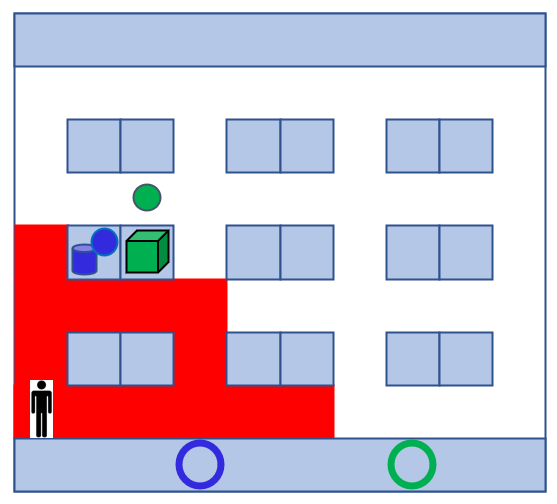
\includegraphics[scale=0.35]{figures/HITL1_case2_a.png}
    \caption{ケース2\ 状態$a$}
    \label{fig:HITL1_case2_a}
\end{figure}

\begin{figure}[!t]
    \centering
    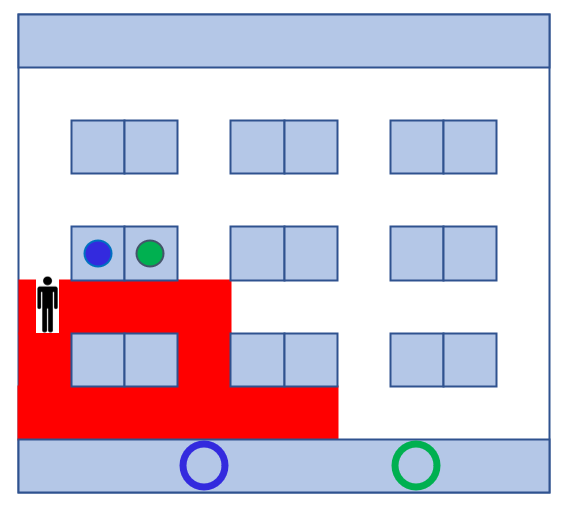
\includegraphics[scale=0.35]{figures/HITL1_case2_b.png}
    \caption{ケース2\ 状態$b$}
    \label{fig:HITL1_case2_b}
\end{figure}

図\ref{fig:HITL1_case2_b}のとき(協調作業が完了した後),人間がもとの作業場所に戻っていく.ロボット1,2は遷移先が人間の経路で進入禁止エリアになっているので,人間のゴール地点で安全が確認されるまで遷移は禁止される.

$H$が受理状態で自己ループする事象が生起したなら,スーパーバイザはロボット同士の衝突を回避する制御のみを行うようになる(図\ref{fig:HITL2_case2_c})

%人間は行動102により右に行くか,行動104により下に行くか2通りの遷移を持っている.102が生起したとき,ロボット1は人間が状態143に到達するまで遷移を禁止され,ロボット2は人間が状態144に遷移するまで行動を禁止される.一方,104が生起した場合,状態42,43が人間の経路から除外されることにより,ロボットの進入禁止エリアは図\ref{fig:human_area_3}のようになる.そのため,ロボット1,2ともに下に遷移することが可能になる. 

\begin{figure}[!t]
    \centering
    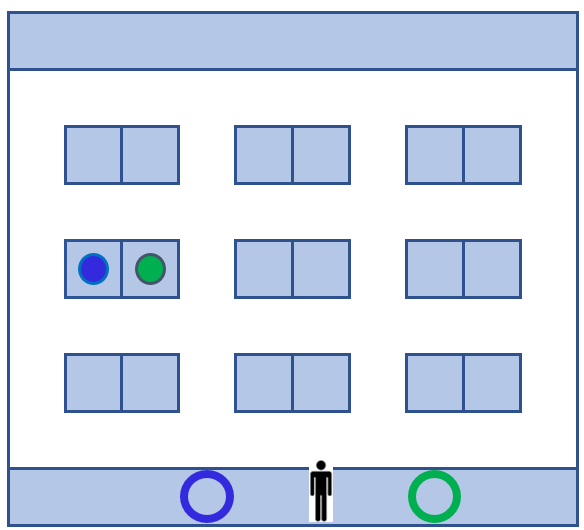
\includegraphics[scale=0.33]{figures/HITL1_case2_c.png}
    \caption{ケース2\ 状態$c$}
    \label{fig:HITL2_case2_c}
\end{figure}


\subsection{方法2}

ケース2でも,最小安全隔離距離は1マスとして,シミュレーションを行う.
先ほどと同じ例を用いて,動的に進入禁止エリアが変化する方法2での制御を考える.
この人間とロボットが協調する例を方法2で考えるとき,注意しなければならない点がある.
ロボット1に割り当てられた荷物の位置にロボットが存在し,協調作業場所(この例では隣のマス)に人間が存在しているときのみ,協調作業が可能である.また,タスクを完遂するには協調作業をするために,人間と人間の協力を必要とするロボット1が,荷物の積み込みをする際に近づかないといけないのである.
%ロボットの隣のマスに人間が存在しているタイミングで協調作業しなければならない.よって,
方法2の制御要求は,mutexという関数を用いて,同時に存在してほしくないロボットの状態と人間の状態の組み合わせを入力し,それらの状態の組を排除する制御要求を与えてスーパーバイザを作成する方法であった.
%ロボットと人間が一定の距離以上近づく事象を禁止するという制御要求がスーパーバイザに与えられる.
この例では,人間とロボットの間に1マス以上の間隔をあける制御要求があるので,スーパーバイザを計算する際に与える制御要求について,人間がロボット1を手伝う作業場所に存在し,ロボット1が目的の商品の場所にいる状態の組みを削除したものを制御要求として与える必要がある.
% この問題を解決しない限り,受理状態に到達するができない.
% 厳密にいえば,人間に接近するロボットの動作だけを禁止するわけではなく,

% つまり,ロボットが商品の場所で荷積みされるのを待っている状態のときその周りを人間が通れなくなってしまう.

しかし,このように制御要求のmutexに与える条件から1組だけ除くだけでは不十分であり,ブロッキング状態に陥る可能性がある.

次に,ブロッキング状態になる可能性がある問題の場面を,ケース2の例とは別の例を用いて紹介する.

図\ref{fig:HITL2_case2_d}のように,人間の助けを必要とするロボットが商品の棚の位置に,その隣に位置する協調作業場所に人間が向かっている場面を想定する.
このとき,人間は協調作業場所へ向かうために左に移動しなければならない.しかし,左に遷移してしまうことで,ロボットと人間が接近しないという制御要求を満たさなくなる.そのため,スーパーバイザに人間が左に遷移する行動を禁止されてしまう.
その結果,ロボットも人間も動くことができずブロッキング状態になる.
人間がそこに行って荷物を積まないと受理状態まで到達できないということで図\ref{fig:HITL2_case2_d}の状態になる前に,ロボットが棚に移動する動作をスーパーバイザが禁止する制御をする.

\begin{figure}[!t]
    \centering
    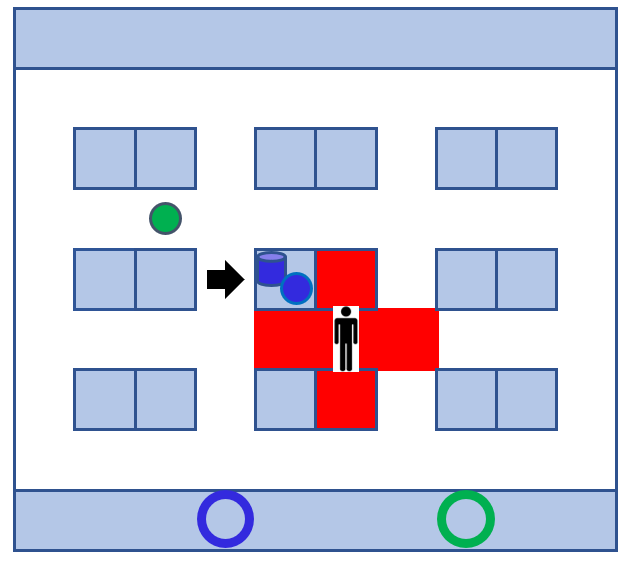
\includegraphics[scale=0.3]{figures/HITL2_case2_d.png}
    \caption{ケース2\ 状態$d$}
    \label{fig:HITL2_case2_d}
\end{figure}

%JIS規格によって,移載が安全に確実に行われるよう,インタロック機能の搭載が義務付けられているので,ロボットを荷物の棚の位置で待機させておくのが望ましいと考えられる.このような理由で,上記のスーパーバイザの制御は理想的でない.

また,その逆に人間が協調作業場所で待機しており,図\ref{fig:HITL2_case2_e}のように,ロボットが人間の周りのマスを経由して荷物の場所に向かっている場合についても同じ問題が生じる.ロボットの右に行く行動が禁止されてブロッキング状態になり,それを回避するため,スーパーバイザは人間が協調作業場所に到着する以前に制御を行うことになる.これは人間の行動を便宜上制御可能であると定義したことによって起こった問題である.

\begin{figure}[!t]
    \centering
    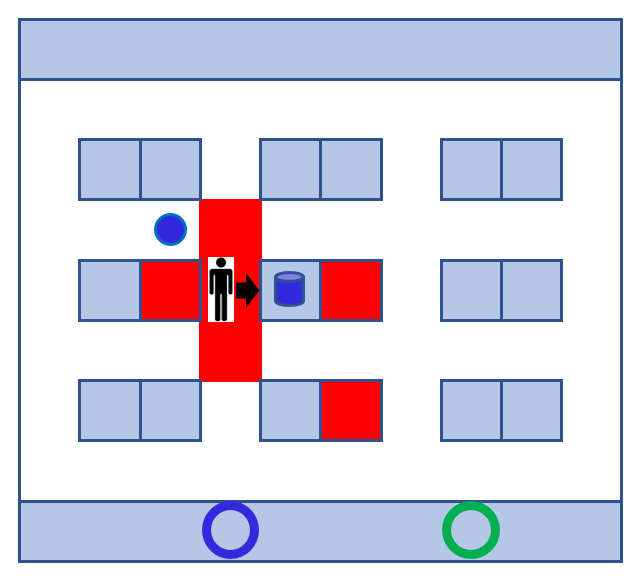
\includegraphics[scale=0.3]{figures/HITL2_case2_e.png}
    \caption{ケース2\ 状態$e$}
    \label{fig:HITL2_case2_e}
\end{figure}

これらを踏まえると,ロボットと人間が協力して積まれる荷物周辺では,制御要求を緩和して,ロボットと人間の接近を許可する制御が求められる.
つまり,協調して積み込む商品の保管場所近くでは,人間とロボットの間に距離をおくという制御要求の一部を削除する方法を提案する.
具体的には,mutexの条件のうち,ロボットが商品の場所に存在している状態を含むペアを削除し,次に人間が協調作業場所に存在している状態を含むペアを削除するといった2つの手順を踏んで考える.

%mutex(G, H, [s_G, s_H])と書き,Gが状態s_Gに,Hが状態s_Hに同時に存在する状態を排除することを意味する.状態のペア[s,s]を条件といい,%

まずは,前者のロボット1が商品を保管する棚である状態$[s_{G,item}]$にいるときの状態の組を除外する.
これはロボットが人間より先に協調作業場所に到着したときを想定した対策である(図\ref{fig:HITL2_case2_robot_waits_human}).

\begin{figure}[!t]
    \centering
    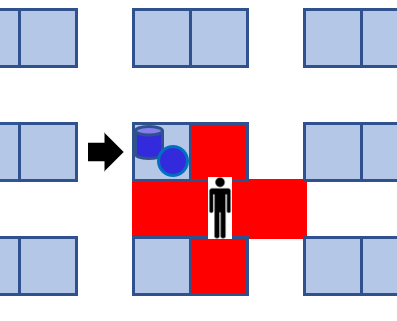
\includegraphics[scale=0.3]{figures/HITL2_case2_robot_waits_human.png}
    \caption{ロボットが待機しているときに発生し得るブロッキング状態}
    \label{fig:HITL2_case2_robot_waits_human}
\end{figure}

%mutexの条件のうち,ロボット側の状態にロボットに割り当てられた商品がある棚の状態が含まれているペアを,1組を除き削除する.削除の対象とならない状態のペアは,ロボットと人間が同じ状態に存在するペアである.

今回のシミュレーションでは,最小安全隔離距離を1マスとおいているので,人間側の状態に該当の位置の周りが含まれた状態のペアだけを削除すればよい.

%$G_1$が割り当てられた商品を保管する棚の状態が条件となっているペアを1組だけ除いて削除する.
商品のある棚の状態を$s_{G,item}$とすると,削除の対象となるのは$[s_{G,item},s_{G,item}-10], [s_{G,item},s_{G,item}-1], [s_{G,item},s_{G,item}+1], [s_{G,item},s_{G,item}+10]$である.
$[s_{G,item},s_{G,item}]$も状態$s_{G,item}$を含んでいる.しかし,ロボットと人間が同じ状態に存在する状態のペア$[s_{G,item},s_{G,item}]$は衝突回避の制御をする上で必要であるから,削除してはいけない.

もし,人間の安全を確保するために2マス以上確保しなければならないという制御要求を与えられていたなら,ロボット1が目的の商品の棚にいるときを含み,$G$と$H$が異なった状態にいるペアを削除することで解決される.

そして後者,人間が待機しているときロボットの経路に人間の周りが含まれていた場合も(図\ref{fig:HITL2_case2_human_waits_robot}),前者同様に,ロボットと人間の状態が同じペアを除いて,人間が協調作業場所にいるすべての状態のペアをmutexの条件から削除する.
%$[s_{H,help}-10,s_{H,help}], [s_{H,help}-1,s_{H,help}], [s_{H,help}+1,s_{H,help}], [s_{H,help}+10,s_{H,help}]$

\begin{figure}[!t]
    \centering
    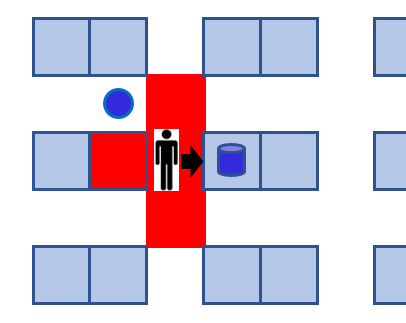
\includegraphics[scale=0.3]{figures/HITL2_case2_human_waits_robot.png}
    \caption{人間が待機しているときに発生し得るブロッキング状態}
    \label{fig:HITL2_case2_human_waits_robot}
\end{figure}

シミュレーションの結果である制御について解説する.

\begin{figure}[!t]
    \centering
    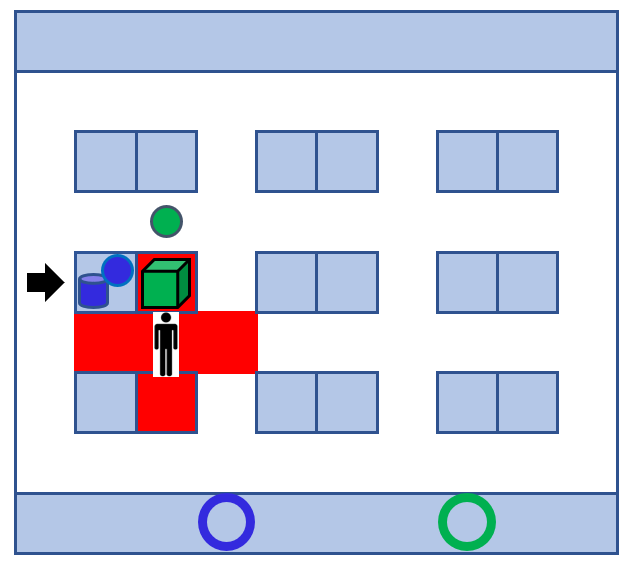
\includegraphics[scale=0.3]{figures/HITL2_case2_f.png}
    \caption{ケース2\ 状態$f$}
    \label{fig:HITL2_case2_f}
\end{figure}
\begin{figure}[!t]
    \centering
    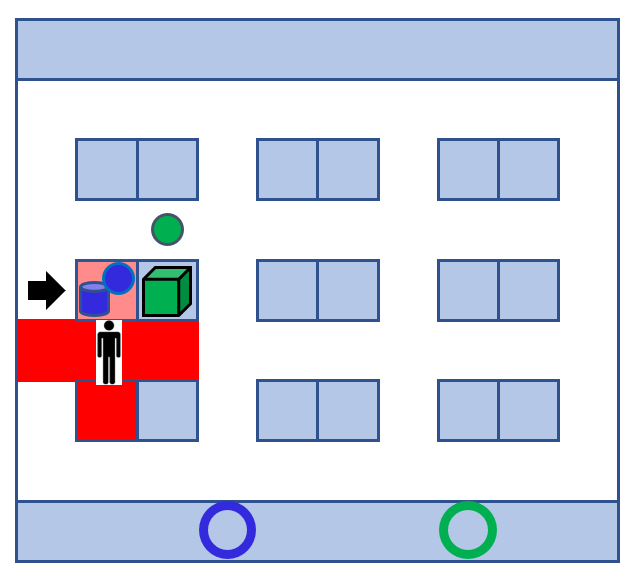
\includegraphics[scale=0.3]{figures/HITL2_case2_g.png}
    \caption{ケース2\ 状態$g$}
    \label{fig:HITL2_case2_g}
\end{figure}

図\ref{fig:HITL2_case2_f}の状態のとき,ロボット1は荷物のある状態32に待機しており,ロボット2は状態23に,人間が状態43に存在している.このとき,人間に荷物を積んでもらうまでロボット1の次に発生する行動は禁止され続ける.ロボット2の遷移先は,人間が近くにいるため進入禁止エリアとされているので,ロボット2の行動25が禁止される.また,$H$がとる可能性があるのは行動107である.ここで,ロボット1と人間に関する制御要求を緩和していることにより,人間の左へ遷移する行動が許されている.人間が左へ遷移したときの進入禁止エリアの変化は図\ref{fig:HITL2_case2_g}のようになる.図\ref{fig:HITL2_case2_g}の色の薄い進入禁止エリアはロボット2だけが対象であり,ロボット1には影響しない.

また,人間が協調作業場所に存在するとき,進入禁止エリアは図\ref{fig:HITL2_case2_h}のように変化する.

\begin{figure}[!t]
    \centering
    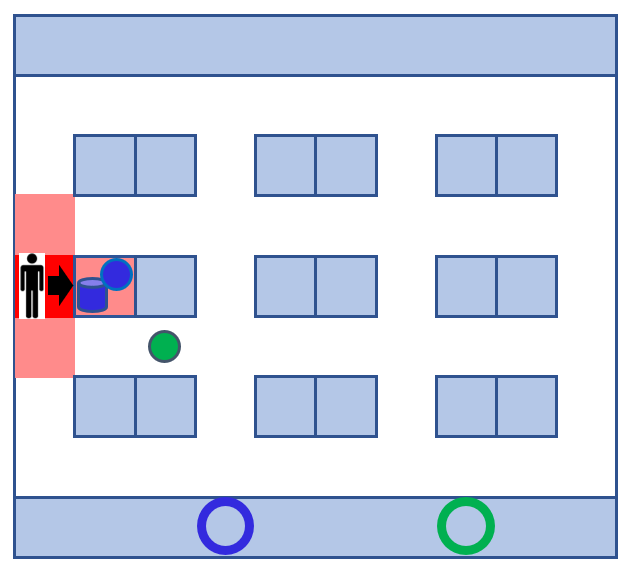
\includegraphics[scale=0.3]{figures/HITL2_case2_h.png}
    \caption{ケース2\ 状態$h$}
    \label{fig:HITL2_case2_h}
\end{figure}

商品の積み込みの作業が終わり,人間が移動すると,再びロボット1,2は人間のまわりに接近を禁止されるようになる(図\ref{fig:HITL2_case2_i}).

\begin{figure}[t]
    \centering
    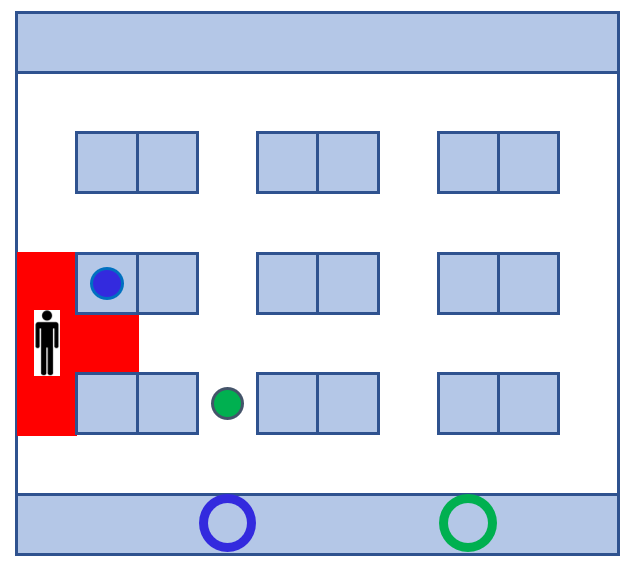
\includegraphics[scale=0.3]{figures/HITL2_case2_i.png}
    \caption{ケース2\ 状態$i$}
    \label{fig:HITL2_case2_i}
\end{figure}


\section{2つの方法の比較}
方法1としてロボットに人間の経路上を使用させない方法,方法2としてロボットを人間に決められた距離より接近させない方法の2つの制御方法によるケーススタディを紹介した.

方法1では,人間の経路に指定されていれば,人間が離れていてもロボットが使用できず,別のルートを通るか待つ必要があった.方法2をもちいると,離れているときは,ロボットが待つことなく走行ができるというメリットがある.

しかし,方法2は方法1に比べて,経路が増加するたびに計算時間も増加する傾向がある(表\ref{tb:run_time}).また,最小安全隔離距離の$d$が増えるにつれ,さらに計算量が増加してしまう.

比較の表について,制御要求を作成して,スーパーバイザの計算が終わるまでの計算時間の50回の平均を示している.また,$G_2$と$H$の状態遷移をそれぞれ経路の分岐が1つ増えるよう図\ref{fig:run_time_G2},\ref{fig:run_time_H}のように変更した.

\begin{table}[htb]
  \begin{tabular}{|l|r|r|r|r|} \hline
    &\ref{sect:case1}節の例 & $G_2$に遷移を追加 & $H$に遷移を追加 & $G_2$と$H$に遷移を追加 \\ \hline
    方法1 & 3.069 & 3.337 & 3.204 & 3.950 \\ \hline
    方法2 & 3.222 & 3.974 & 4.105 & 5.098 \\ \hline
  \end{tabular}
  \caption{計算時間の比較(単位 : 秒)}
  \label{tb:run_time}
\end{table}

\begin{figure}[h]
    \centering
    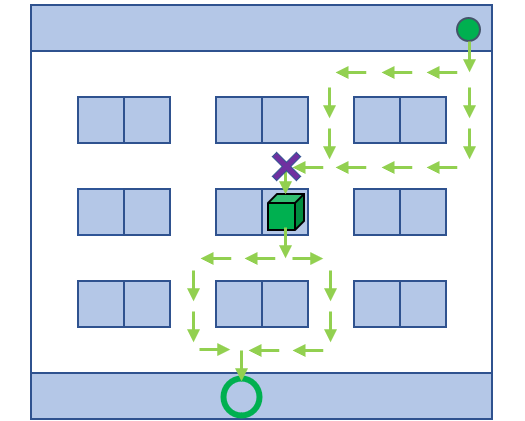
\includegraphics[scale=0.35]{figures/run_time_G2.png}
    \caption{変更後の$G_2$の経路}
    \label{fig:run_time_G2}
\end{figure}

\begin{figure}[h]
    \centering
    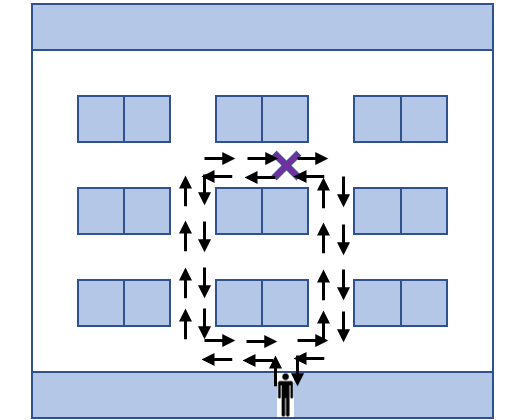
\includegraphics[scale=0.35]{figures/run_time_H.png}
    \caption{変更後の$H$の経路}
    \label{fig:run_time_H}
\end{figure}
\clearpage

% 6.
\chapter{結論}

\section{まとめ}

離散事象システムのスーパーバイザ制御理論を用いて,倉庫の自動化を考える上で,倉庫内に人間が立ち入る際に人間の安全が保障されたロボット制御方法を2つ提案した.
1つは人間の使用する通路にロボットを侵入させない方法で,もう1つはロボットが決められた値以上人間に接近しないように,動的にロボットが入ることができない範囲を定める方法であった.

また,予期せぬトラブルが発生したときの対処と人間とロボットが倉庫内で協調作業をするケーススタディによって,提案した方法が有効であることを検証した.

そしてこれらの方法をもちいることで,人が倉庫内に行かなければならないとき,人間をシステムの一部として制御し,倉庫の自動化システムを稼働させたまま人間が立ち入ることができ,ロボットの無駄な待ち時間を削減し,作業効率の向上をもたらす.


\section{今後の課題}

オンライン制御をもちいて,トラブルをランダムなタイミングで発生させても対応できるように改良を加えると,より実用的なシステムになるので,オンライン制御での実装は今後の課題とする.

また,ロボット台数および人間の人数が少ないケースでは見えなかった問題が,エージェントの数を増やすことによって浮き彫りになる可能性が考えられる.今回の研究では,ロボット2台,人間1人よりエージェントを増やしたシミュレーションを行うことができなかった.これは計算量が膨大になってしまい,今回使用したTCTの計算方法の限界であることが原因である.そこでSemi-Model Free\cite{Semi-Model_Free}を用いることで問題が解決されると考えられる.
\clearpage

% 謝辞
\begin{acknowledgment}
本論文の執筆にあたり,多くの方々にご支援いただきました.
中間報告会および審査会では,阿多信吾教授,岡育生教授,辻岡哲夫准教授,蔡凱准教授より,貴重なご指導とご助言を賜り,深く感謝申し上げます.
特に,主指導教員である蔡凱准教授には,研究の進め方や枠組みにおいて,丁寧かつ熱心なご指導をいただきました.心より感謝申し上げます.

最後に,研究について有益なご討論,ご助言をいただきました同研究学科の皆様にお礼申し上げます.

ありがとうございました.
\end{acknowledgment}

% Reference
\thesisbib

\end{document}